\chapter{Phase portraits of autonomous vector fields}

\begin{definition}\label{def:2.1}
	The \textbf{phase portrait} of an autonomous vector field $ v (x) $ on a manifold $ M $ is the partition of $ M $ into the phase curves of this field.
\end{definition}

Phase curves are of three types:
\begin{enumerate}[(i)]
	\item equilibrium points, i.e., degenerated curves corresponding to fixed solutions;
	\item embedded intervals (bounded or not); i.e., the images $\varphi(I)$ of the solutions of $\varphi :I\longmapsto M$, which are embedded;
	\item \textbf{closed phase curves} (embedded circles) corresponding to \textbf{periodic solutions} $\varphi :$
	\begin{equation}
	\label{2.1}
	\varphi (t+T)=\varphi (t),\text{ \ \ }t\in \mathbb{R},
	\end{equation}
	where $ T> 0 $ is the expansion \textbf{period} (we assume that this is the minimum period satisfying \eqref{2.1}).
\end{enumerate}

Throughout this chapter we only consider autonomous vector fields; therefore, we will leave the adjective `autonomous'.

\begin{example} (Mathematical pendulum).\label{example:2.2}
	This is the following system
	$$
	\dot{x}=y,\text{ \ \ }\dot{y}=-\sin x
	$$
	over phase space $M=\mathbb{S}^{1}\times \mathbb{R}$ (cylinder).
	\begin{figure}[!ht]
		\centering
		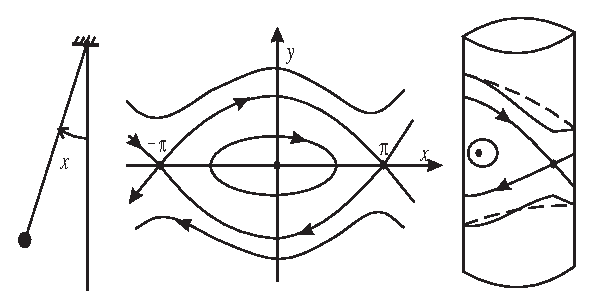
\includegraphics [scale=1.1]{jtr21}
		\caption{Pendulum.}
		\label{fig:2.1}
	\end{figure}
	
	It is easy to see that the function 
	\begin{equation}
	\label{2.2}
	H=\frac{1}{2}y^{2}-\cos x
	\end{equation}
	is the first integral of this system, i.e., $ \dot {H} \equiv 0 $. Notice the following properties of $ H: $
	\begin{itemize}
		\item point $\left( 0,0\right) $ is an absolute minimum point and $ H (0,0) = -1 $;
		\item point $\left( \pi ,0\right) $ is a saddle point and $ H (\pi, 0) = 1 $;
		\item $H(x,y)\rightarrow \infty $ as $\left\vert y\right\vert
		\rightarrow \infty $.
	\end{itemize}

It is also easy to see that, in addition to the above equilibrium points, we have two phase curves of type (ii); these are the separatrices of the saddle point $\left( \pi ,0\right) $ lying in the level $\left\{ H=1\right\}$. The remaining phase curves are closed and can be divided into two groups: (a) around the equilibrium point $(0,0)$ (corresponding to fluctuations of limited
amplitude) and (b) circulating cylinder (they correspond to the pendulum spinning around the anchor point).

We can calculate the periods of the above periodic solutions lying on the level $ H = h $ of the first integral. We have $ dt = dx / y$, where $ y $ is given by formula \eqref{2.2}: $y=\pm \sqrt{2(h+\cos x)}$. So in case (a) we have
$$
T=2\int_{x_{1}}^{x_{2}}\frac{dx}{\sqrt{2(h+\cos x)}},
$$
where $ x_ {1,2} $ are two zeros of function $ h + \cos x $. Here, from $ x_ {1} $ to $ x_ {2} $, the trajectory length is $ y> 0 $, but for symmetry it is exactly half the period. In case (b) we have
$$
T=\int_{0}^{2\pi }\frac{dx}{\sqrt{2(h+\cos x)}}.
$$

Unfortunately, the above can not be counted in terms of elementary functions. In fact, after substituting $ u = \cos x $ (with $ dx = du / \sin x = -du / \sqrt {1-u ^ {2}}) $ we get 
$$
T=4\int_{-h}^{1}\frac{du}{\sqrt{(1-u^{2})(h+u)}}.
$$
The right side of the last equation is the called \textit {elliptic integral} defining a certain elliptic function\footnote{Ellipses and elliptic functions appear very often in differential equations of classical mechanics (see \cite{Ar3}).} (Task 2.45).

We also notice that the closed phase curves in this example are not isolated, they are in whole families.
\end{example}

\section{Periodic solutions}

Closed phase curves are also called periodic trajectories or periodic orbits. In Example \ref{example:2.2}, they exist in whole families, but there are also periodic trajectories isolated.

\begin{definition}
	An isolated closed phase curve of an autonomous vector field is called  \textbf{limit cycle}.
	
	The equilibrium point of such a field, which is surrounded by non-isolated closed phase curves, is called \textbf {center}.
\end{definition}

\begin{example}\label{example:2.4}
	Let's consider the system
	$$
	\dot{x}=x(1-x^{2}-y^{2})+y,\text{ \ \ }\dot{y}=-x+y(1-x^{2}-y^{2}).
	$$
	It is convenient to change this system in a polar coordinate system $\left( r,\varphi \right) $%
	$$
	\dot{r}=r(1-r^{2}),\text{ \ \ }\dot{\varphi}=-1
	$$
	(Task 2.47). Easily, the solutions starting with $ r = r_ {0} \in \left (0,1 \right) $ increase with time to $ r = 1 $ and solutions starting with $ r_ {0}> $ 1 are reduced to $ r = 1 $. The starting solution from $ r_ {0} = 1 $ is constant and corresponds to the isolated solution on the $ XY $ plane (see Figure \ref{fig:2.2}).
\end{example}

\begin{figure}[!ht]
	\centering
	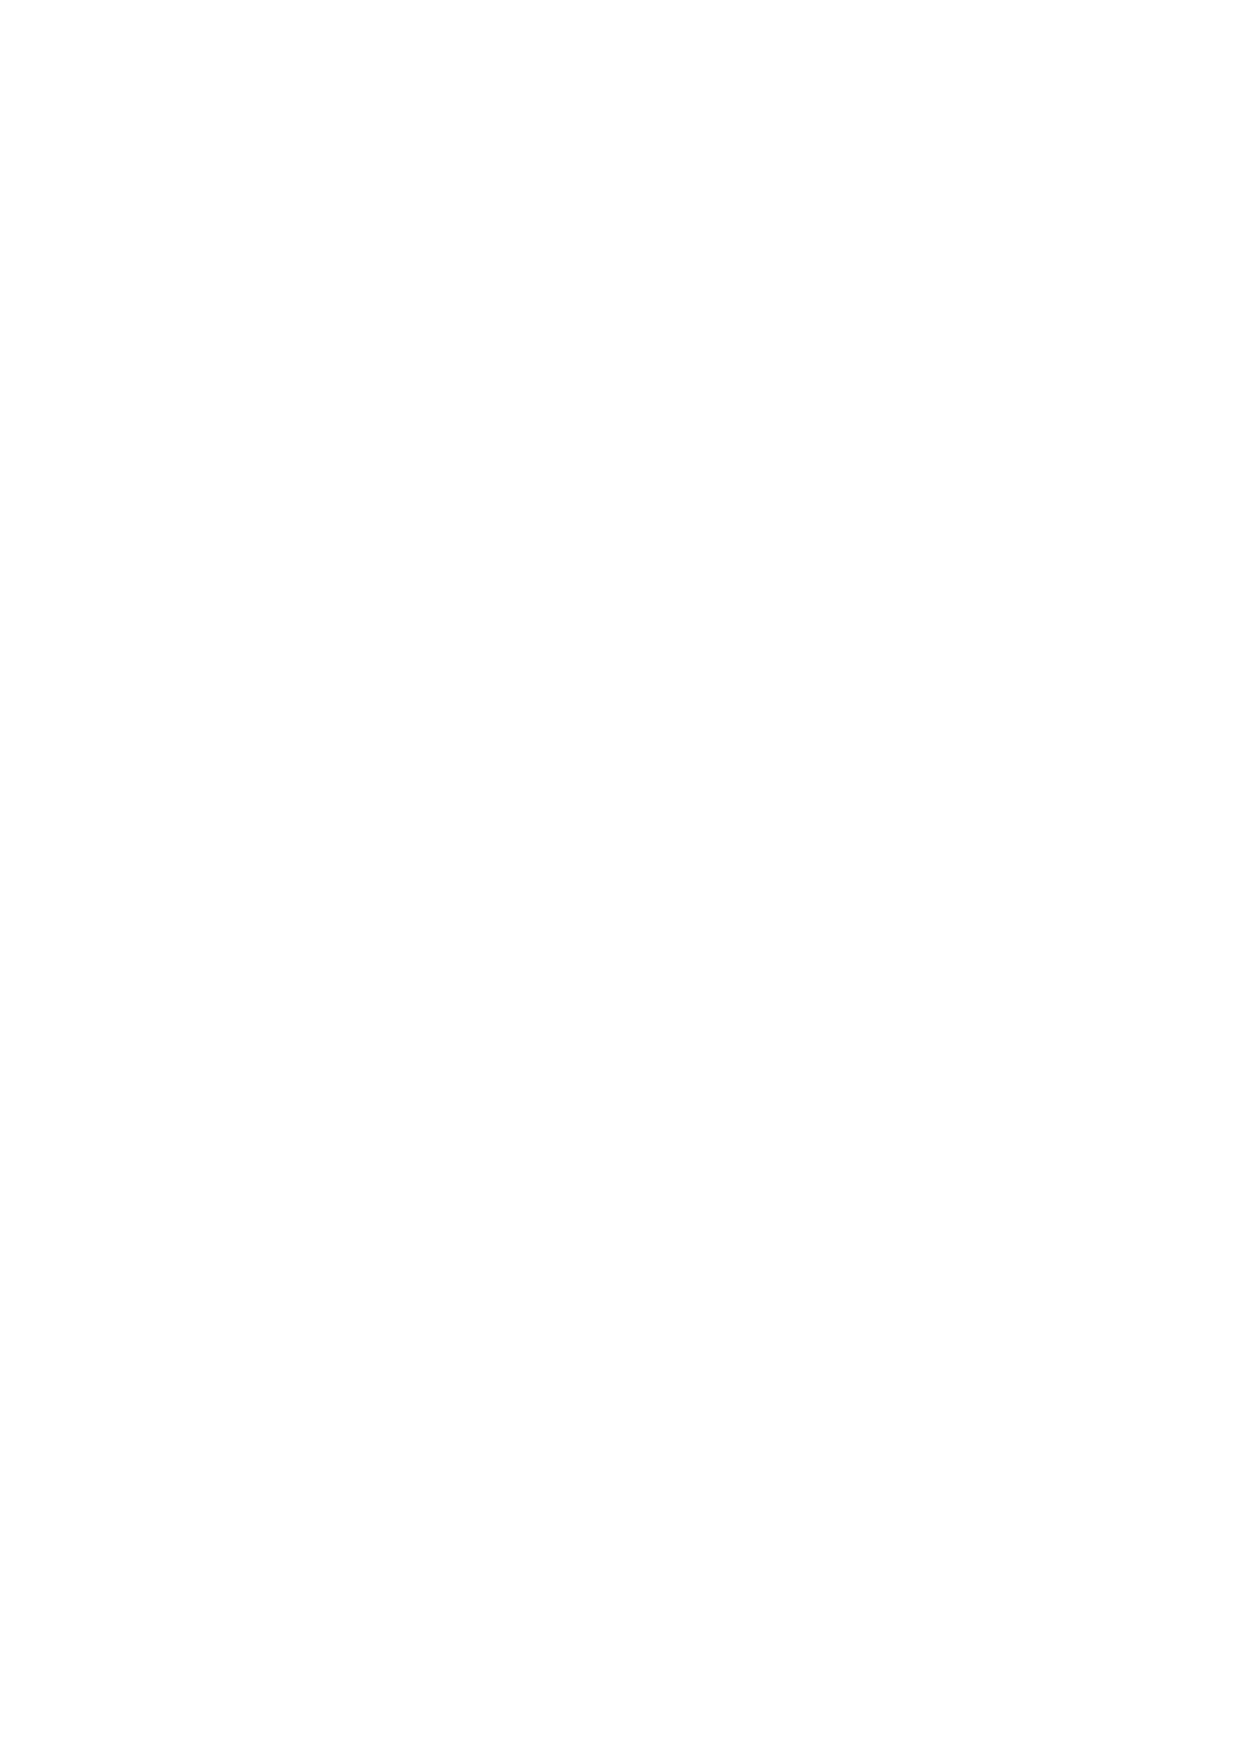
\includegraphics [scale=1]{jtr22}
	\caption{Limit cycle.}
	\label{fig:2.2}
\end{figure}

\begin{definition}
	Let $ \gamma $ be a closed phase curve of a vector field in $ M $. Take a section $ S $ (from `section' we mean \textbf{cutting}) of the transversal hyperplane (i.e. at a non-zero angle) to $ \gamma $ at a certain point $ p_ {0} \in \gamma $. From point $x_{0}\in S$ starts the solution $\varphi
	(t;x_{0})$, which after some time $ T (x_ {0}) $ returns to $ S $, $\varphi (T(x_{0});x_{0})\in S$. The resulting mapping $f:S\longmapsto S$ (diffeomorphism with the right domain): $$
	x_{0}\longmapsto f(x_{0})=\varphi (T(x_{0});x_{0})
	$$
	 is called the \textbf{Poincaré return map} (see Figure \ref{fig:2.3}).
\end{definition}

\begin{figure}[!ht]
	\centering
	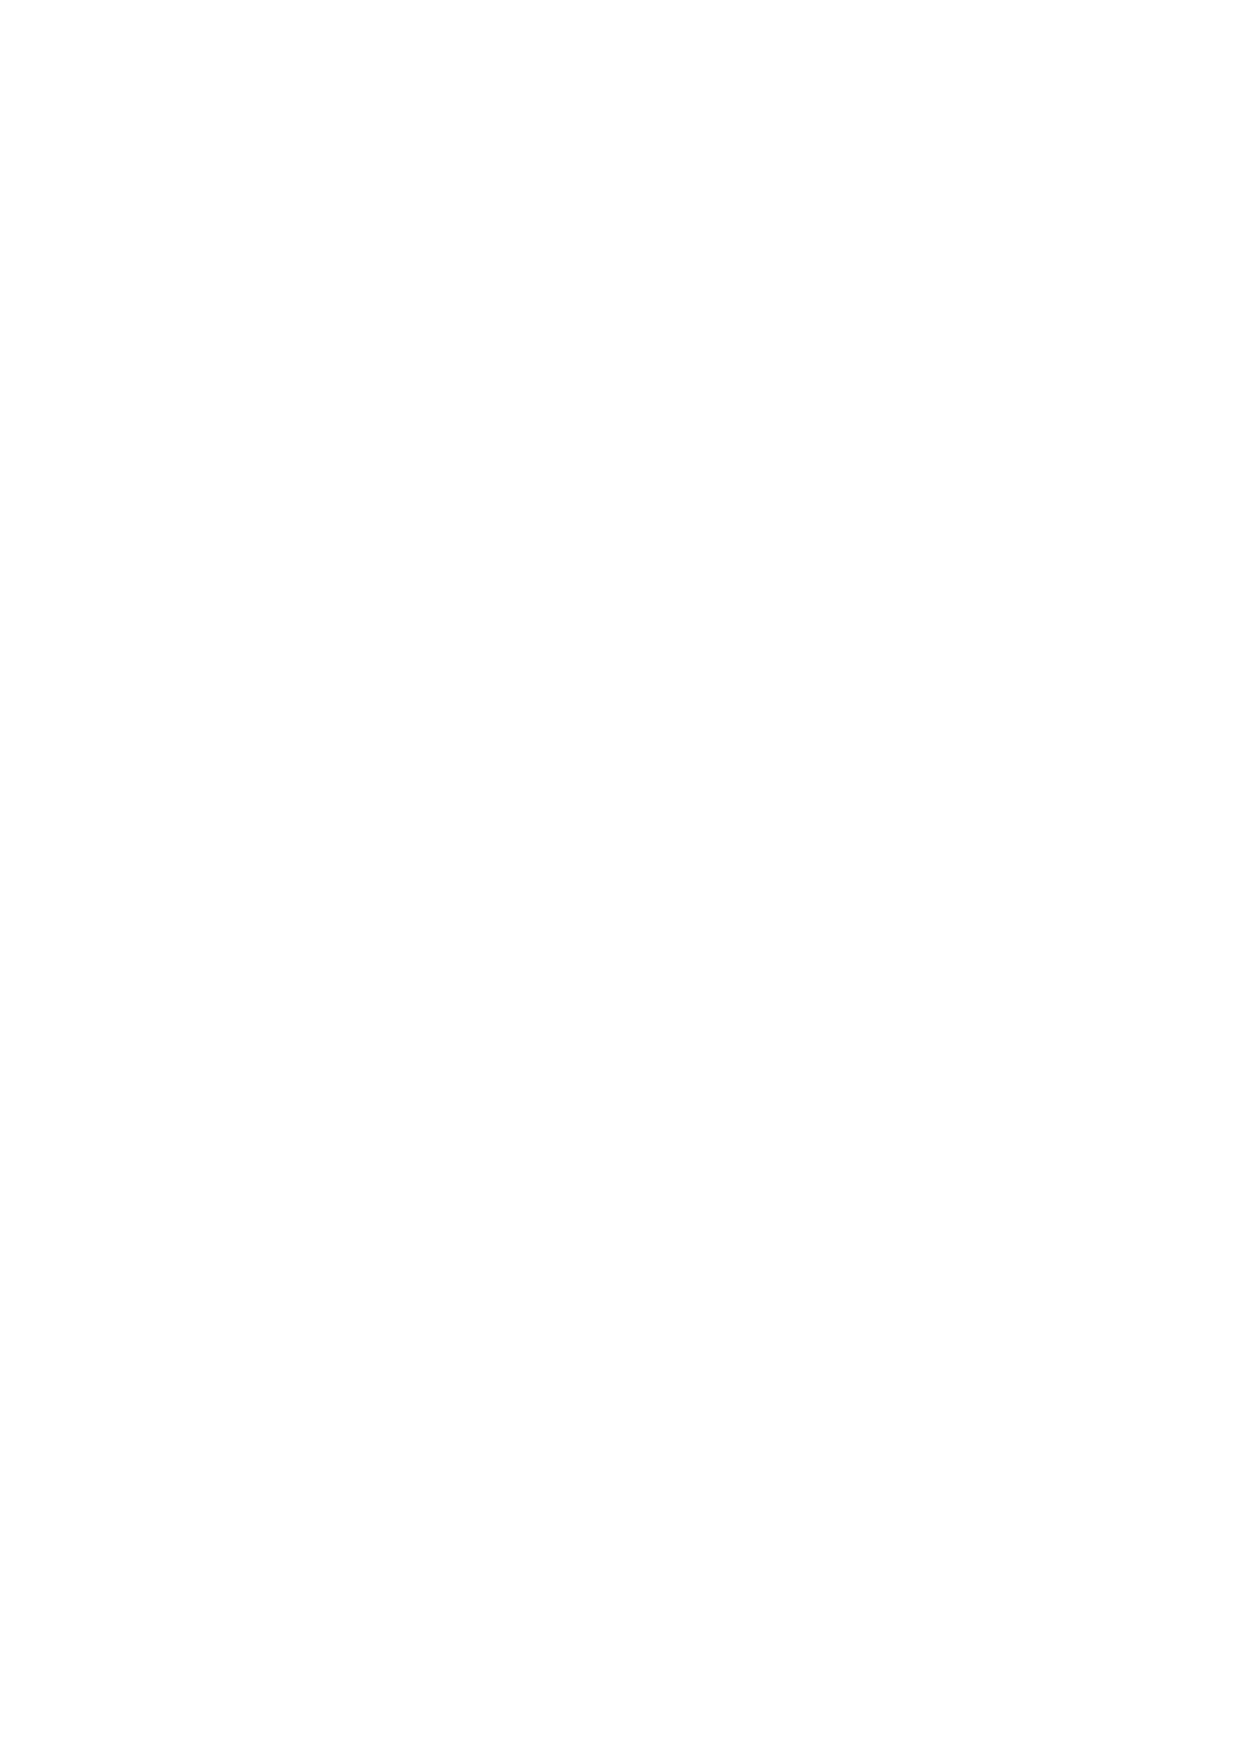
\includegraphics [scale=1]{jtr23}
	\caption{Return map.}
	\label{fig:2.3}
\end{figure}

In this definition, there is a significant arbitrariness associated with the choice of the cutting $ S $. It turns out that this is not a big problem because if $f^{\prime }:S^{\prime }\longmapsto S^{\prime }$ is the return map associated with another cutting $ S ^ {\prime} $, there is the following

\begin{lemma}
	The $f$ and $f'$ diffeomorphisms are conjugated by a certain diffeomorphism of the same class of smoothness as $f$ and $f'$.
	\begin{proof}
		Let $ f_ {1}: S \longmapsto S ^ {\prime} $ and $ f_ {2}: S ^ {\prime} \longmapsto S $ be the natural maps along the solution. We have $f=f_{2}\circ f_{1}$ and $f^{\prime }=f_{1}\circ f_{2}$.
	\end{proof}
\end{lemma}

The cuting $(S, p_0)$ can be identified with $ \left (\mathbb {R} ^ {n-1}, 0 \right)$, where $ n = \dim M $,  and the return map defines the germ of the diffeomorphism $ f: \left (\mathbb {R} ^ {n-1}, 0 \right) \longmapsto \left (\mathbb {R} ^ {n-1}, 0 \right ) $ (since $f(p_{0})=p_{0}$) of form
$$
f(z)=Az+\ldots
$$
(Task 2.48).

\begin{definition}
	The closed curve $ \gamma $ is \textbf{hyperbolic} if the fixed point $ z = 0 $ for the above diffeomorphism is hyperbolic, i.e., $ \left \vert \lambda _ {j} \right \vert \not = 1 $  for the eigenvalues of matrix $ A $.
\end{definition}

The following two propositions are simple analogues of the Lyapunov Theorem and the Hadamard-Perron Theorem.

\begin{proposition}
	If $ \left \vert \lambda _ {j} \right \vert <1 $ for all eigenvalues, the curve $ \gamma $ is asymptotically stable, i.e., any solution $ \varphi (t) $ starting close enough to $ \gamma $ has the property that \emph{dist}$ \left (\varphi (t \right), \gamma) \rightarrow 0 $ as $ t \rightarrow \infty $.
\end{proposition}

\begin{proposition}
	If the curve $ \gamma $ is hyperbolic, then there exist invariant submanifolds $ W ^ {s} $ (stable) and $ W ^ {u} $ (unstable) such that \emph{dist}$ \left (g ^ {t} (x), \gamma \right) \rightarrow 0 $ for $x\in W^{s}$ when $ t \rightarrow \infty $ and \emph{dist}$ \left (g ^ {t} (y), \gamma \right) \rightarrow 0 $ for $ y \in W ^ {u} $ when $ t \rightarrow - \infty $.
\end{proposition}

More interesting is the following

\begin{proposition}
	If $ n = \dim M = 2 $ and both the manifold and the vector field $ v (x) $ are analytic and $ \gamma $ is a closed phase curve of $ v $, then either $\gamma$ is a limit cycle, or there exists (unambiguously) a first integral in a neighborhood of the $ \gamma $ curve.
	\begin{proof}
		In fact, here we have to prove that the periodic solutions of $ v $ can not accumulate on the $ \gamma $ curve. This is equivalent to the fact that the transformation of Poincaré's return $ f: \left (\mathbb {R}, 0 \right) \longmapsto \left (\mathbb {R}, 0 \right) $ has either a fixed point in $z=0$ or $f(z)\equiv z$. But it follows from the analytic function of $ f (z) -z $ (assuming that $ S $ is analytic) and the standard properties of analytic functions.
		In the case of $ f = id $, all the phase curves in the neighborhood of $ \gamma $ are closed and they are the levels of the first integral of $ F $ for the vector field (Figure \ref{fig:2.4}).
	\end{proof}
\end{proposition}

\begin{figure}[!ht]
		\centering
		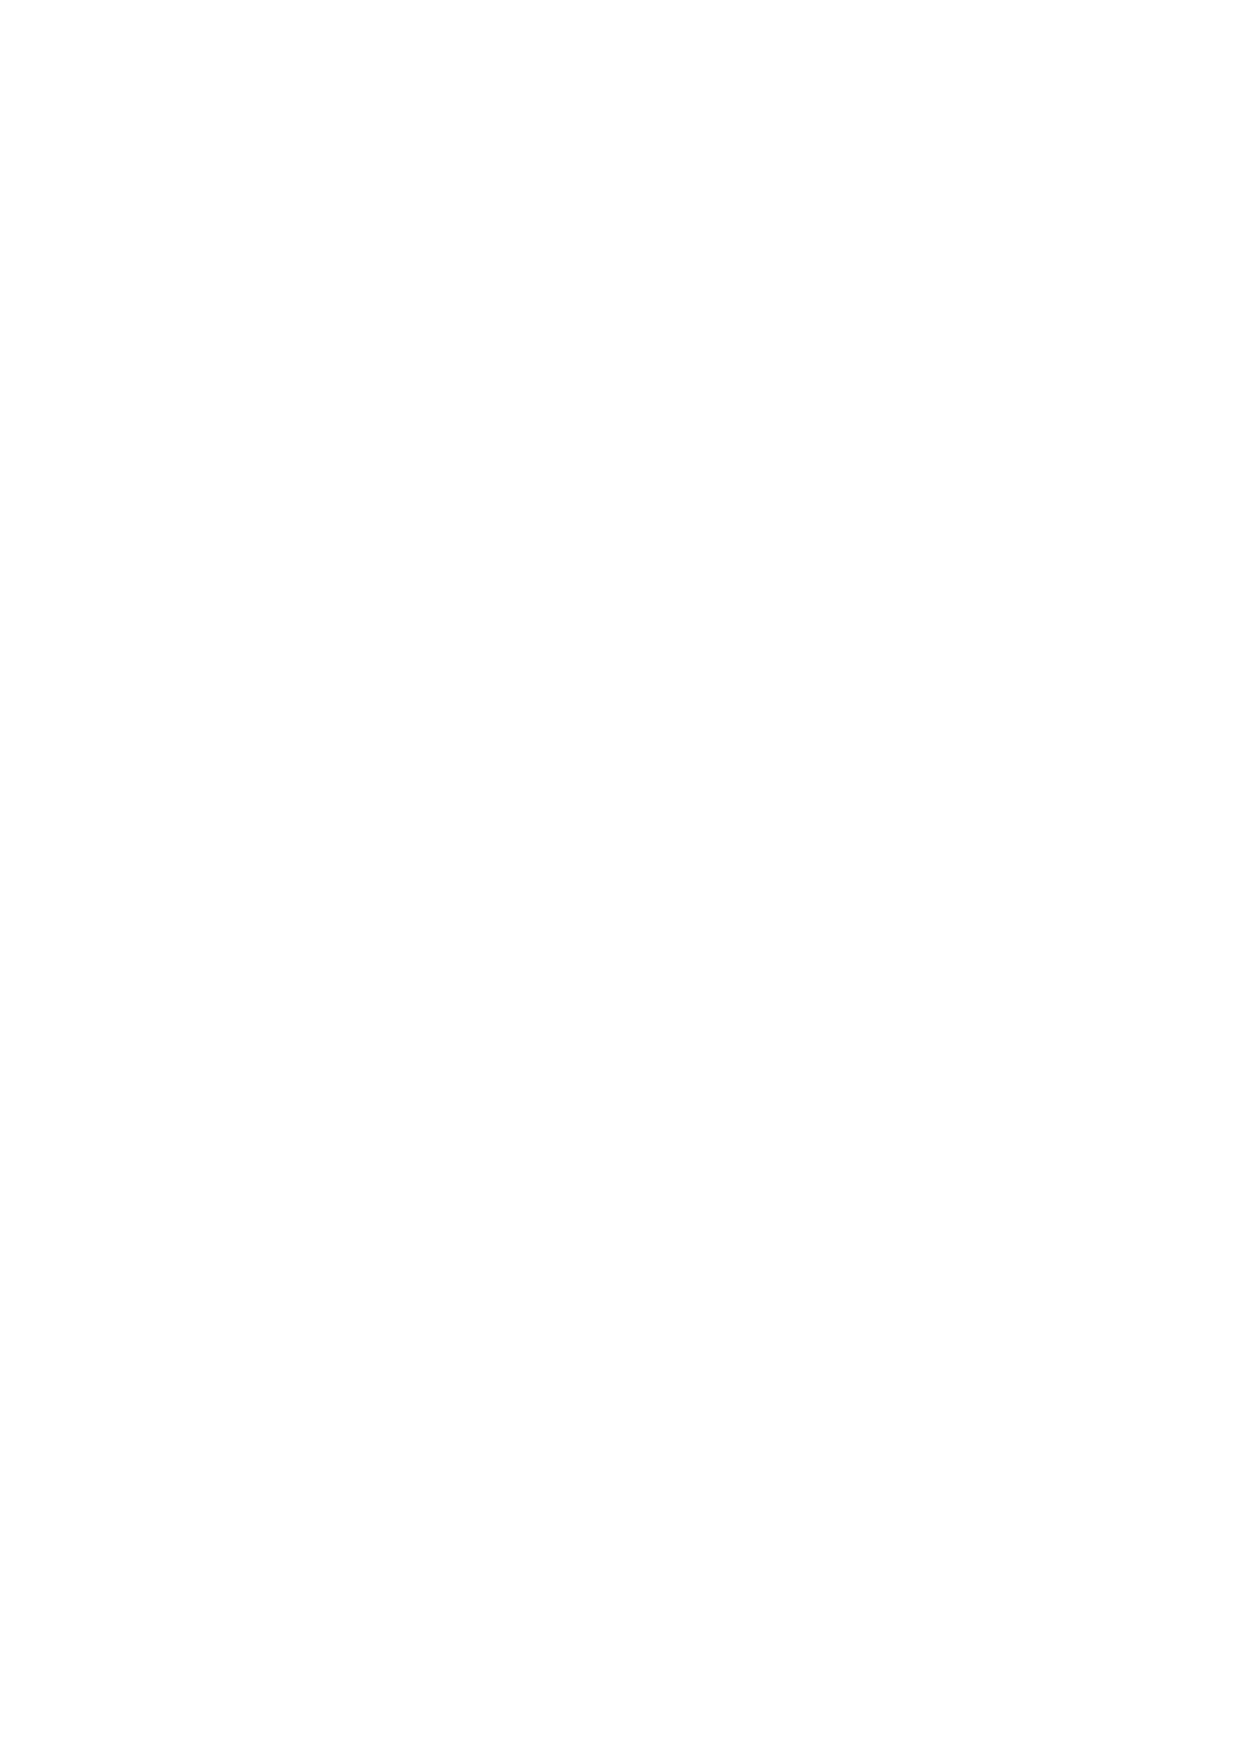
\includegraphics [scale=1.1]{jtr24}
		\caption{First integral levels.}
		\label{fig:2.4}
\end{figure}

This statement has an analogy for the singular point $ x = y = 0 $ of the analytic vector field if the linear part of the field has imaginary eigenvalues, i.e., \begin{equation}
\label{2.3}
\dot{x}=\alpha x-\omega y+\ldots ,\text{ \ \ }\dot{y}=\omega x+\alpha
y+\ldots ,\text{ \ }\omega \not=0
\end{equation}

\begin{proposition}\label{prop:2.11}
	In the case of an analytical field of type \eqref{2.3}, there is one of the two following possibilities: either point $ \left (0,0 \right) $ is a focus (stable or unstable) or there exists (unambiguously) a first integral in a neighborhood of this point (i.e. $ \left (0, 0 \right) $ is a center).
	\begin{proof}
		We have to change to the polar coordinate system $ \left (r, \varphi \right) $. We will get
		\begin{equation}
		\label{2.4}
		\dot{r}=\alpha r+r^{2}A(r,\varphi ),\text{ \ }\dot{\varphi}=\omega
		+rB(r,\varphi ),
		\end{equation}
		where $A(r,\varphi )$ and $B(r,\varphi )$ develop into a coherent power series from $r$ with coefficients that are trigonometric polynomials of $ \varphi $ (Task 2.49). The phase curves of this system satisfy the differential equation
		\begin{equation}
		\label{2.5}
		\frac{dr}{d\varphi }=r\frac{\alpha +rA(r,\varphi )}{\omega +rB(r,\varphi )}.
		\end{equation}
		Its solutions $r=\psi (\varphi ;r_{0})$, such that $\psi
		(0;r_{0})=r_{0}$, transforms
		$$
		f:\left( \mathbb{R}_{+},0\right) \longmapsto \left( \mathbb{R}_{+},0\right) ,%
		\text{ \ \ }r_{0}\longmapsto \psi (2\pi ;r_{0}),
		$$
		which is analogous to the Poincaré's return map. In essence, this is a return map for the field \eqref{2.3} from the semicircle $ S _+ = \left \{\left(x, 0 \right): x \geq 0 \right \} \simeq \mathbb {R} _ {+}$ in itself (see Figure \ref{fig:2.5}). From the convergence of the series representing $ A $ and $ B $, the transformation of $ f $ is analytic.
	\begin{figure}[!ht]
		\centering
		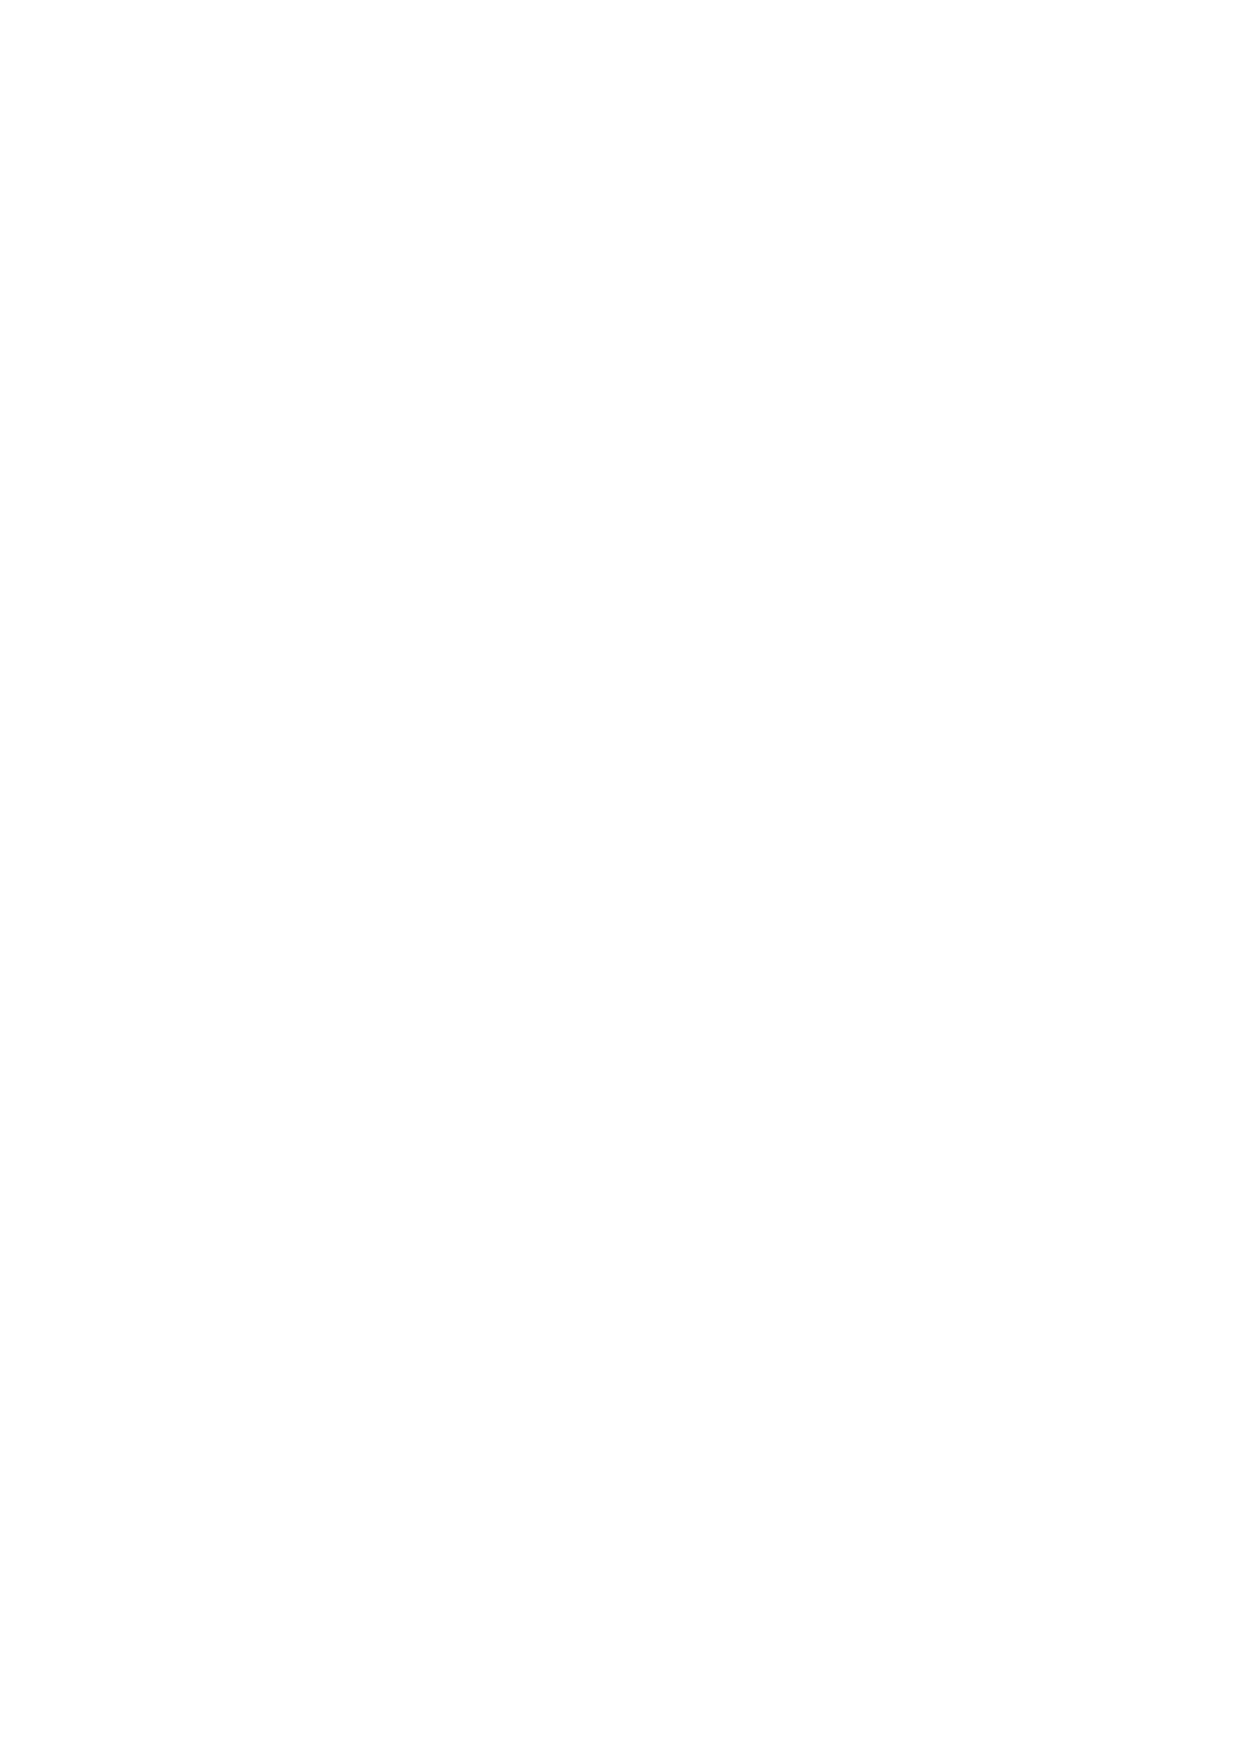
\includegraphics [scale=1]{jtr25}
		\caption{Return map.}
		\label{fig:2.5}
	\end{figure}
		The fixed points of the diffeomorphism $ f $ correspond to the closed  phase curve of the field \eqref{2.3}. As in the proof of the previous statement, either $ r = 0 $ is an isolated fixed point for $ f $ or $ f = id $ and then all the phase curves in the neighborhood of $ x = y = 0 $ are closed.
	\end{proof}
\end{proposition}

The Poincaré return map expands $ f $ into the series
\begin{equation}
\label{2.6}
f(r)=a_{1}r+a_{2}r^{2}+\ldots
\end{equation}
It is easy to see that $a_{1}=\exp \left( 2\pi \alpha /\omega \right)$ (Task 2.50).

\begin{lemma}
	If $a_{1}=1$ then $a_{2}=0$ and, more generally, if $a_{1}-1=a_{2}=\ldots =a_{2k-1}=0$ then $a_{2k}=0$.
\end{lemma}

This lemma is a consequence of the Poincaré-Dulac Theorem (commanded in Chapter \ref{subsec:3.3.1}) and therefore we do not prove it here.
The reader can prove it by using some symmetry properties ($ \varphi \longmapsto \varphi + \pi)$ for the functions $ A $ and $ B $ at \eqref{2.4}.

Hence, if $ a_ {1} -1 = a_ {3} = a_ {5} = \ldots = a_ {2k-1} = 0 $ and $ a_ {2k+1}>0$ (respectively $<0$) the point $ x = y = 0 $ is a stable focus (respectively unstable).
	
\begin{definition}\label{def:2.13}
	The coefficients
	$$
	c_{1}=\frac{\omega }{2\pi }(a_{1}-1),\text{ \ }c_{3}=\frac{\omega }{2\pi }%
	a_{3},\text{ \ }c_{5}=\frac{\omega }{2\pi }a_{5},\ldots
	$$
	are called \textbf{Poincaré-Lyapunov focal quantities}.
\end{definition}

\begin{remark}
	Focal quantities are important when examining the so-called \emph{small limit cycles}, i.e., those that arise from the focus when the vector field depends on certain parameters. But they are difficult to count. Here are some ways to calculate them; this way was in fact used by Lyapunov.
	
	Instead of real coordinates, we will use the coordinates $ z = x + iy $ and $ \bar {z} = x-iy $, $ i = \sqrt {-1}, $ so that the vector field is written in the form of one complex equation
	\begin{equation}
	\label{2.7}
	\dot{z}=iz+Az^{2}+Bz\bar{z}+C\bar{z}^{2}+Dz^{3}+Ez^{2}\bar{z}+Fz\bar{z}^{2}+G%
	\bar{z}^{3}+\ldots ,
	\end{equation}
	where $ A, B, C, D, E, F, G, \ldots $ are constants fixed. Let's note that the linear part is much simpler here; in particular, $ c_ {1} = 0 $.
	
	We will search for the first one for the equation \eqref{2.7} in the form
	\begin{equation}
	\label{2.8}
	H(z,\bar{z})=z\bar{z}+a_{30}z^{3}+a_{21}z^{2}\bar{z}+a_{12}z\bar{z}%
	^{2}+a_{03}\bar{z}^{3}+\ldots ,
	\end{equation}
	where the condition of reality of $H$ leads to the conditions $a_{ji}=\bar{a}
	_{ij}$. Of course, there will generally be no first integral and the obstacles to that are related to the Poincaré-Lyapunov focal quantities.
	
	The expected $ \dot {H} \equiv 0 $ leads to the following set of algebraic equations
	$$
	(3ia_{30}+\bar{C})z^{3}+(ia_{21}+A+\bar{B})z^{2}\bar{z}\equiv 0
	$$
	for the coefficients of the polynomial $ H $ for the cubic terms. We find $a_{30}=i\bar{C}/3$, $a_{21}=i(A+\bar{B})$ and $H=z\bar{z}	+i\left( C\bar{z}^{3}-\bar{C}z^{3}\right) /3+i\left( \left( \bar{A}+B\right)
	z\bar{z}^{2}-\left( A+\bar{B}\right) z^{2}\bar{z}\right) +\ldots $ (there are no obstacles here). But for the term at $ z ^ {2} \bar {z} ^ {2} $, after scaling the function \eqref{2.8}, we get
	$$
	0\cdot ia_{22}+E+\bar{E}+i(\bar{A}\bar{B}-AB)=0.
	$$
	We see that for $ \dot {H} = 0 $ (modulo of the fifth order), there must be 
	$$
	\Im(AB)+\Re E=0;
	$$
	we expect that the focal quantity $ c_ {3} $ is proportional to $ \textrm {Im} (AB) + \textrm {Re} E $.
	
	To find the constant of proportionality, note that $\dot{\varphi}=1+O(r)$, $H = r^{2}+O(r^{3})$ and
	$\dot{H}=2\left( \textrm{Im}AB+\textrm{Re}E\right) r^{4}+O(r^{5})$. Then
	$$
	f(r)-r=\Delta r\approx \frac{dr}{dH}\Delta H\approx \frac{1}{2r}%
	\int_{0}^{2\pi }\dot{H}d\varphi \approx \frac{2(\textrm{Im}AB+\textrm{Re}E)r^{4}%
	}{2r}\cdot 2\pi .
	$$
	This gives
	\begin{equation}
	\label{2.9}
	c_{3}=\textrm{Im}(AB)+\textrm{Re}E
	\end{equation}%
	(Task 2.51).
\end{remark}

\section{Poincaré-Bendixson criterion}

The problem of detecting limit cycles turns out to be very difficult. This is demonstrated by the following unresolved problem.

\begin{figure}[!ht]
	\centering
	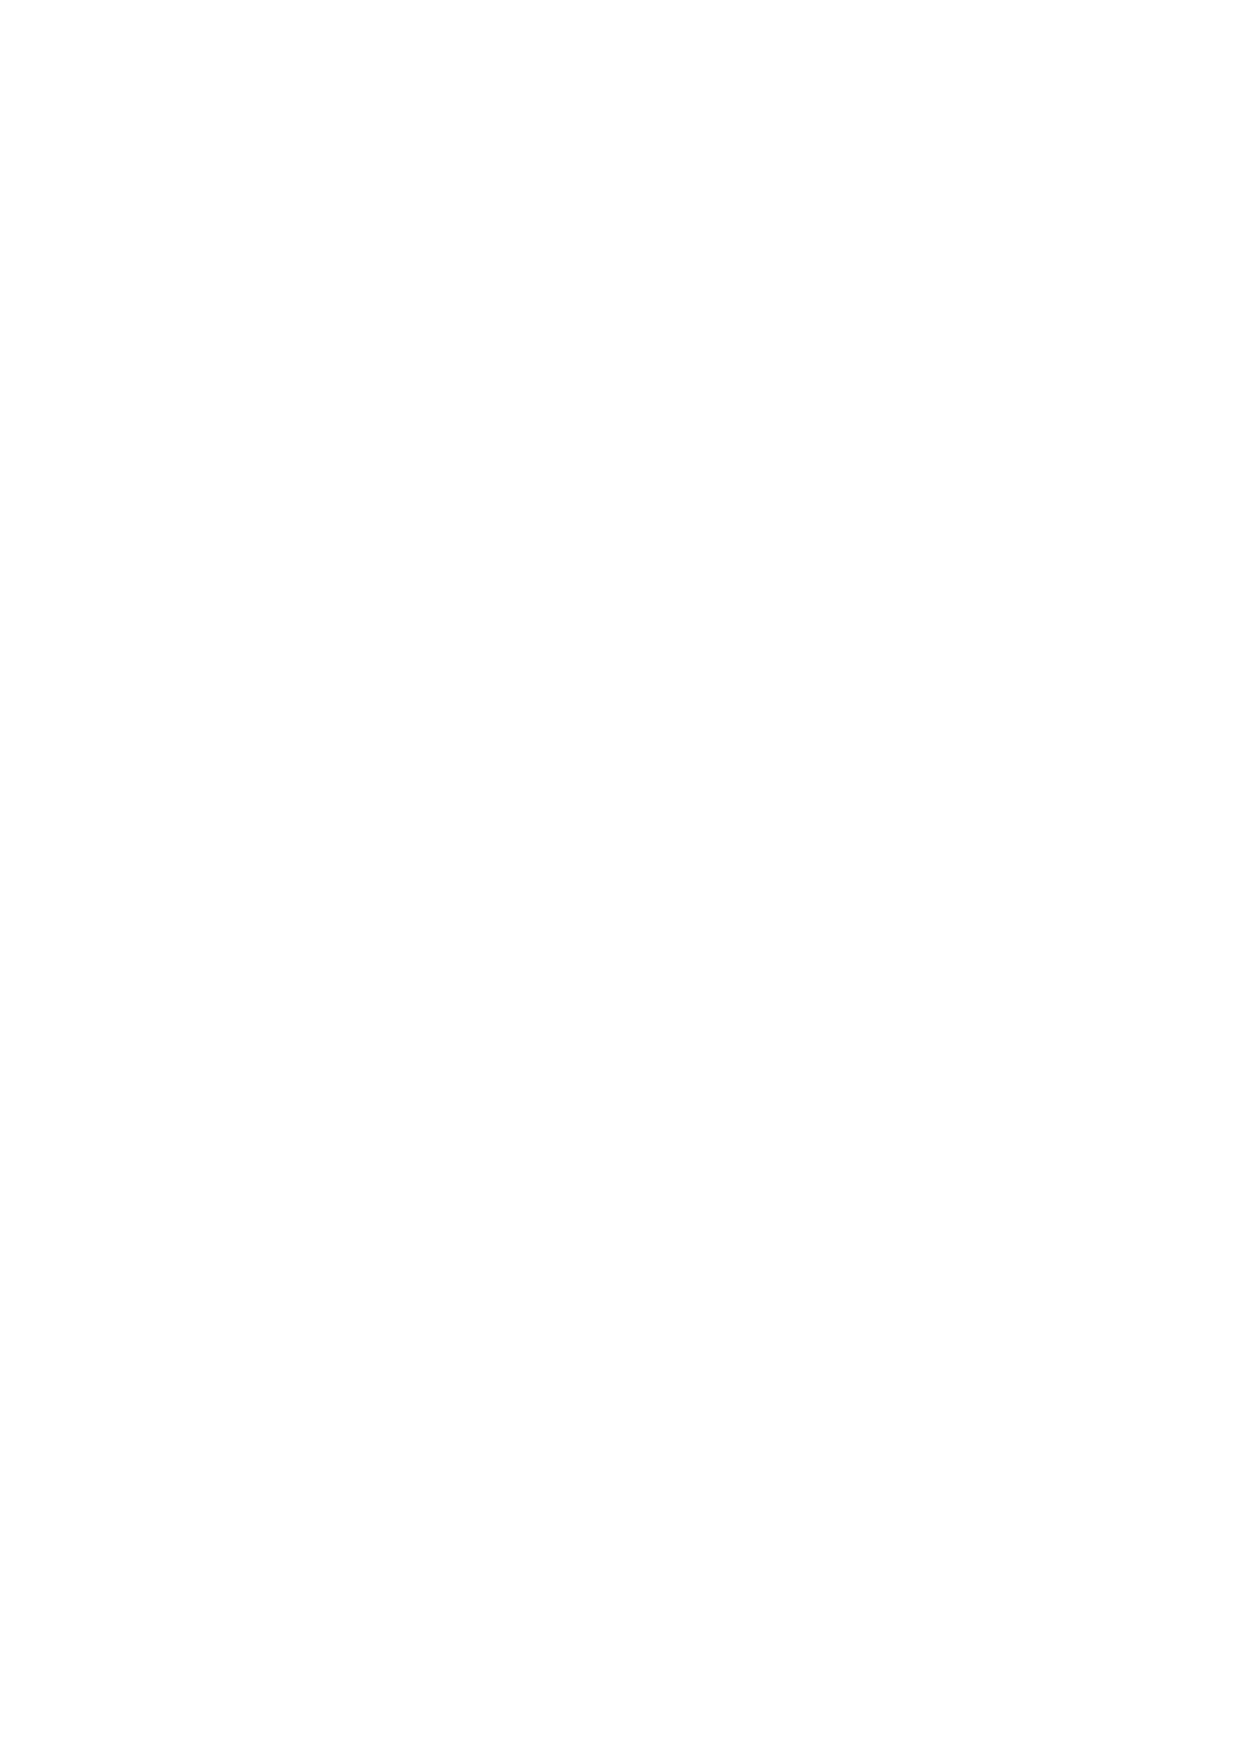
\includegraphics [scale=1.2]{jtr26}
	\caption{Absorbing ring.}
	\label{fig:2.6}
\end{figure}

\begin{hypothesis}(Hilbert's sixteenth problem).\footnote{In essence, this is the second part of the 16th Hilbert's problem. The first part deals with the number and position of congruent components (the so-called ovals) for real algebraic curves of the form $ F (x, y) = 0 $. Here the problem is largely solved (with appropriate generalizations).}
	Give an estimate in terms of degrees of polynomials $ P $ and $ Q $ for the number of polynomial cycles of the vector field of form
	\begin{equation}
	\label{2.10}
	\dot{x}=P(x,y),\text{ \ \ }\dot{y}=Q(x,y).
	\end{equation}
\end{hypothesis}

\begin{remark}
	It is known that the number of cycles for a single character field \eqref{2.10} is finite (Yu. Ilyashenko and J. Ecalle), but it is not known if there is a limit of $ n = \max (\deg P, \deg Q) $. There are examples of square boxes with 4 limit cycles (Task 2.52).
\end{remark}

Therefore, concrete methods showing the existence of limit cycles are important. The Poincaré-Bendixson criterion below guarantees us the existence of at least one boundary cycle provided, when the vector field is analytic (see Statement \eqref{2.10}).

Let us assume that we have a vector field of $ v (x) $ on the plane and an area $\mathcal{R}\subset \mathbb{R}^{2}$ of ring type (as in Figure \ref{fig:2.6}) with the following properties:
\begin{itemize}
	\item the field $ v (x) $ has no equilibrium points in $ \mathcal {R} $,
	\item the field  $ v (x) $ on the boundary $ \partial \mathcal {R} $ of the ring $\mathcal {R} $ is directed to the inside of the ring.
\end{itemize}

\begin{theorem}\emph{(Poincaré-Bendixson).}\label{theo:2.17}
	Under these assumptions inside $ \mathcal {R} $, there is at least one closed phase curve of the field $ v $.
\end{theorem}

\begin{figure}[!ht]
	\centering
	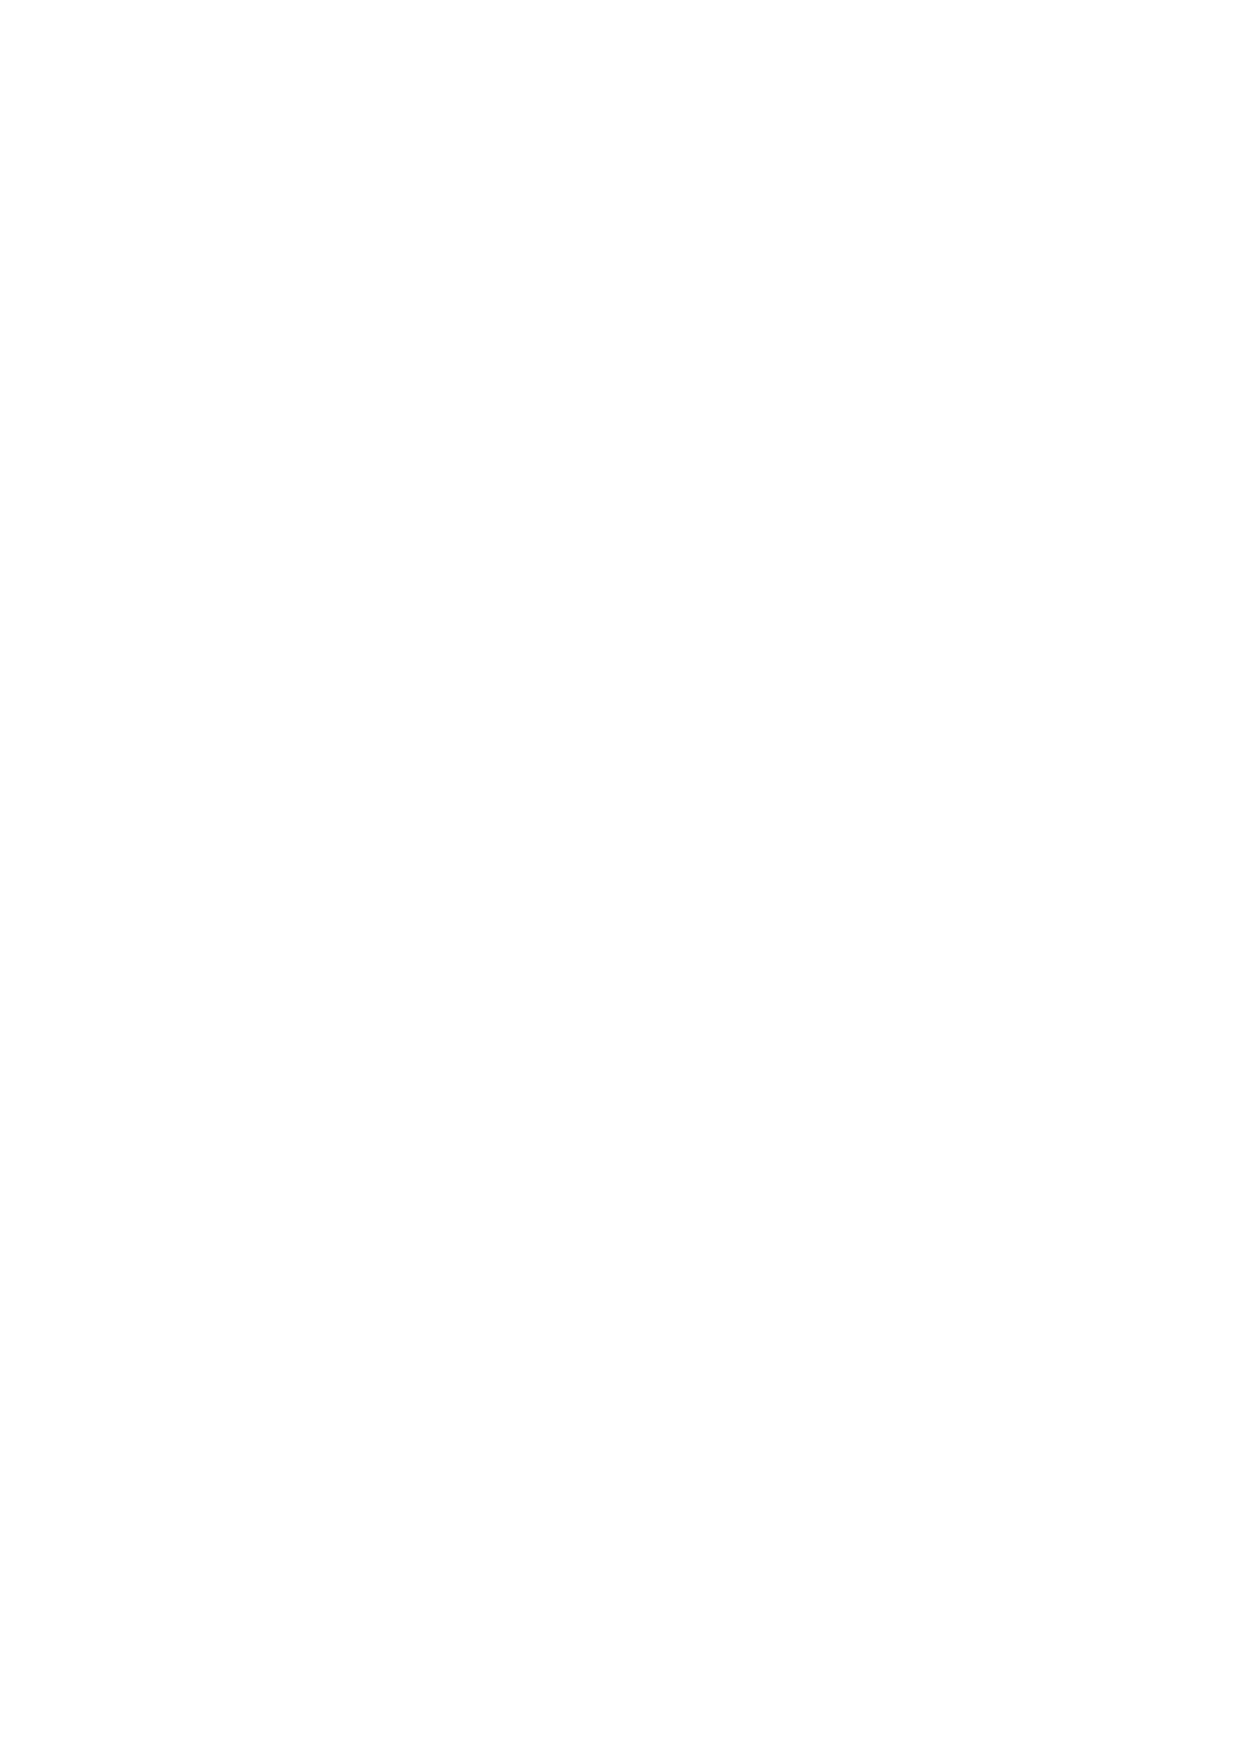
\includegraphics [scale=1.05]{jtr27}
	\caption{Next returns.}
	\label{fig:2.7}
\end{figure}

The proof of this theorem is based on the following important concept in Dynamic Systems.

\begin{definition}
	The \textbf{$\omega$-limit set of the point $x$}, denoted by $\omega(x)$, with respect to the phase flow $g^t$ (or a cascade $\{f^n\}$) is the set of accumulation points of the positive orbit of this point, i.e.,
	$$
	\omega (x)=\left\{ y:\exists t_{k}\rightarrow +\infty \text{ such that }%
	g^{t_{k}}(x)\rightarrow y\right\}
	$$
	(or $\omega (x)=\left\{ y:\exists n_{k}\rightarrow \infty \text{ such that } f^{n_{k}}(x)\rightarrow y\right\} $). (Task 2.53).
	
	In the case of accumulation points of the negative orbit of point $x$, we refer to it as the \textbf{$\alpha$-limit set of the point $ x $}.
\end{definition}

Obviously, the attractive limit cycle is the $ \omega$-limit set at any point lying close to this cycle. There is a version of Poincaré-Bendixson's Theorem that uses the notions of the $\omega $-limit set for the phase flow generated by the vector field $ v $.

\begin{theorem}\label{theo:2.19}
	If for a vector field $ v $ in $ \mathbb {R} ^ {2} $ and a point $ x $ the set $ \omega (x) $ is:
	\begin{enumerate}[(a)]
		\item bounded and
		\item does not include equilibrium points of the field,
	\end{enumerate}
	then $ \omega (x) $ is a closed phase curve of this field.
	\begin{proof}
		Let $ y \in \omega (x) $. We will show that the trajectory of the field passing through $ y $ is closed. To do this, let's choose a local cut (section) $ S $ perpendicular to $ v (y) $ in $ y $. Let us consider the intersection points $ x_ {k} = g_ {v} ^ {t_ {k}} (x) $, $ t_ {k + 1}> t_ {k} $, orbits $ \left \{g_ {v} ^ t (x) \right \} _ {t> 0} $ with the cutting $ S$. The assumption of such points is infinitely many and we can assume that the sequence $ \left \{x_ {k} \right \} $ is monotonous on $ S $ (here we use the fact that we are on the plane) (Task 2.54). So we have the situation as in Figure \ref{fig:2.7}. Let us also note that the entire orbit of $ \Gamma (y) = \left \{g ^ {t} (y): t \geq 0 \right \} $ point $ y $ lies in the set $ \omega (x) $; so we have
		$$
		\omega (y)\subset \omega (x).
		$$
		Of course, $ \omega (y) $ is a closed set, bounded, and without equilibrium points from field $ v $.
		
		Let us assume that the $ \Gamma (y) $ curve is not a closed phase curve. Then $ \omega (y) \not = \Gamma (y) $ and there exists a focus point $z\in \omega (y)\setminus \Gamma (y)$ on the $ \Gamma (y) $ trajectory. Again, we can take the cut $ S_ {1} $ perpendicular to $ v (z) $ in $ z $ and (possibly replacing $y$ with $y_{k}$ points in the intersection of $\Gamma (y)$ with $S_{1}$) obtain the situation as in Figure \ref{fig:2.8}.
		
		\begin{figure}[!ht]
			\centering
			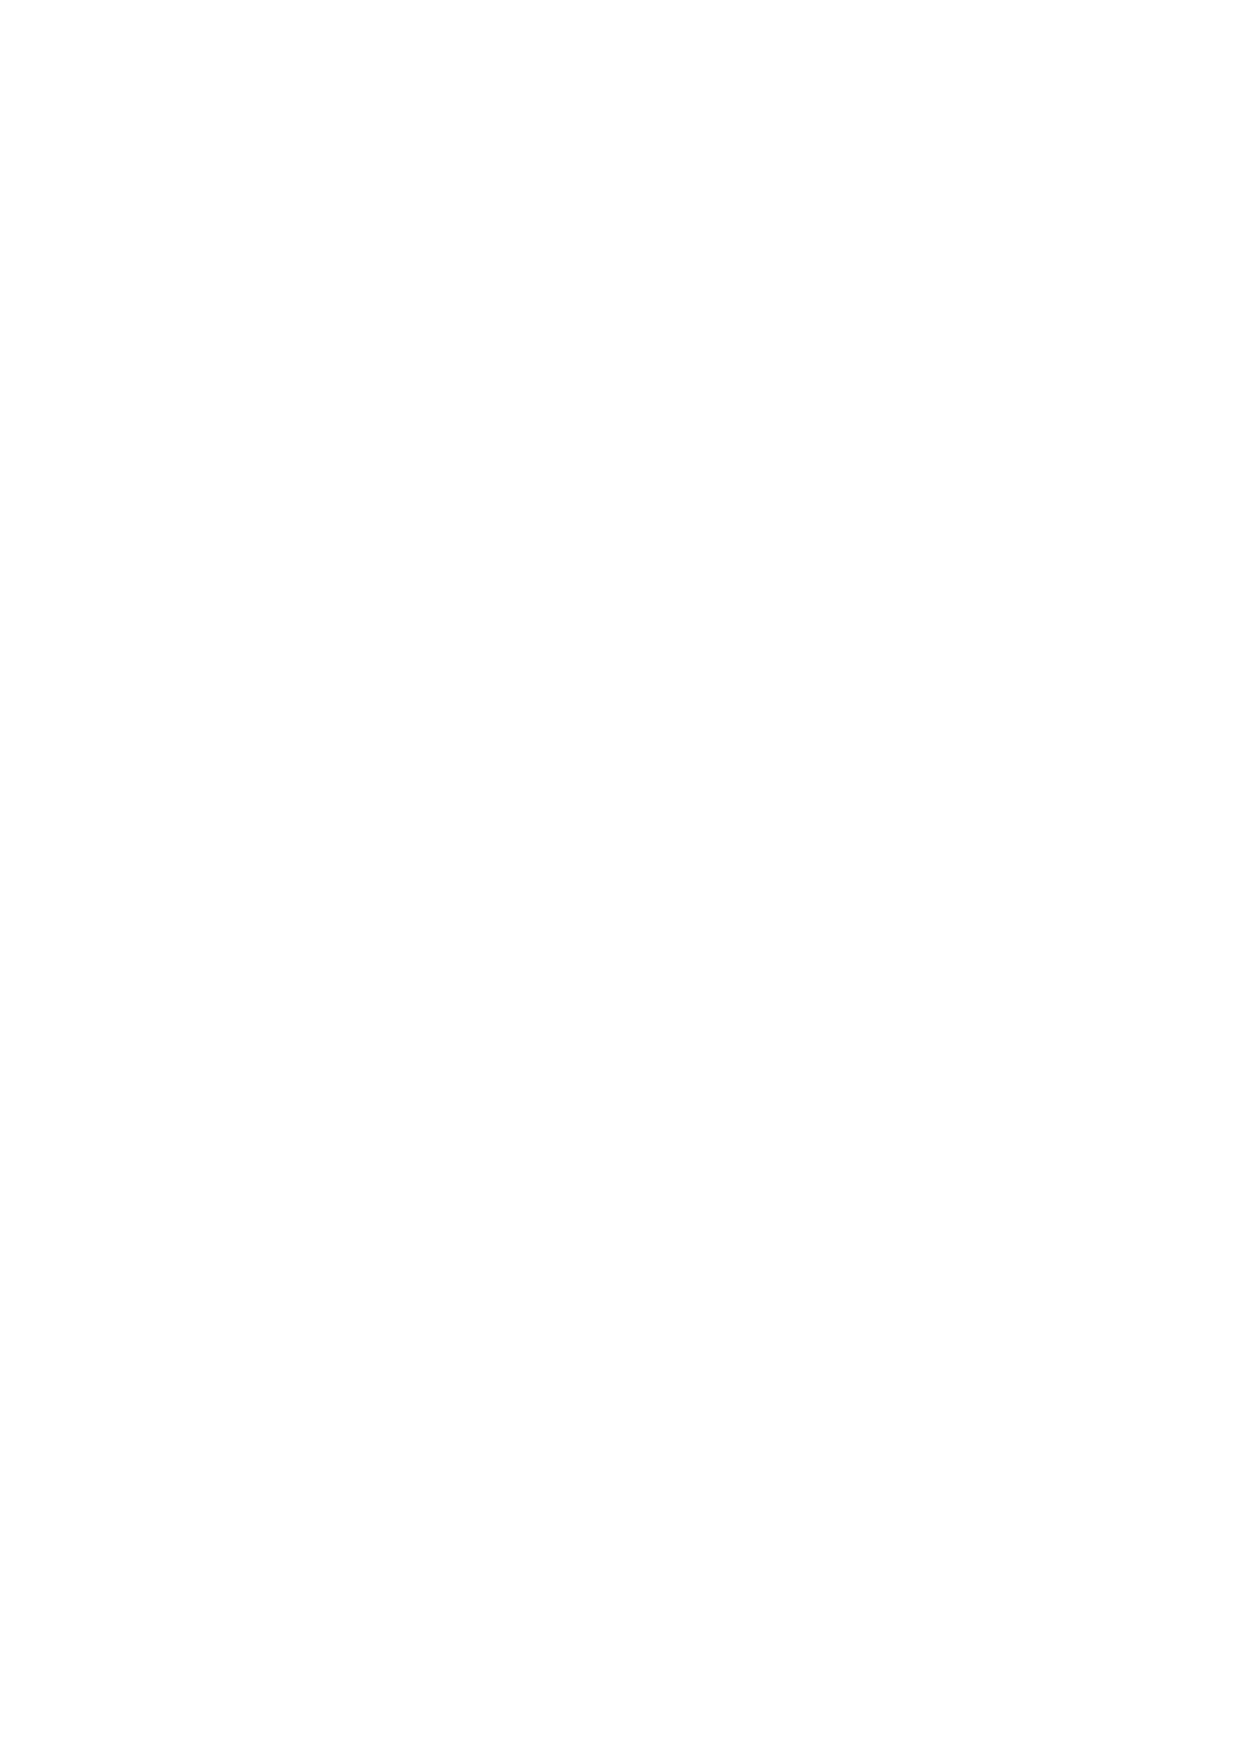
\includegraphics [scale=1.05]{jtr28}
			\caption{Proof of Theorem \ref{theo:2.19}.}
			\label{fig:2.8}
		\end{figure}
	
		Now by deforming the slice of the trajectory $\Gamma (y)$ (from $ y $ to $ y_ {1}) $ so that the new curve is set to the $ v $ field at an angle,we get the area $ \Omega \subset \mathbb {R} ^ {2} $ to which field `enters'. But that gives a contradiction, because it must be $\Gamma (y)\subset \Omega $, and hence, that
		$$
		\omega (x)\subset \Omega ;
		$$
		note that $ \omega (x) $ must also contain the points of the orbit $\left\{ g^{t}(y):t<0\right\} $ of the point  $ y $ outside $ \Omega $.
	\end{proof}
\end{theorem}

\begin{proof}[Proof of the Theorem \ref{theo:2.17}]
	We take any point $ x \in \partial \mathcal {R} $. Then its $ \omega$-limit set satisfies the assumptions of Theorem \ref{theo:2.19}.
\end{proof}

\begin{example}\footnote{This example comes from the monograph \textquotedblleft Modern Geometry\textquotedblright\ by Dubrovin, Novikov and Fomenko. Unfortunately there are not some significant details that I have completed. In addition, Liénard's system usually assumes the form of $ \dot {x} = y $, $ \dot {y} = -f(x)y - g (x) $ or $\dot{x} = y + F(x)$, $\dot{y} = -g(x)$. The system \eqref{2.11} after replacing $ x $ with $ y $ is reduced to the second one.} \label{example:2.20}
	Let's consider the following case, the so-called \emph{Liénard system}
	\begin{equation}
	\label{2.11}
	\dot{x}=y,\text{ \ \ }\dot{y}=-x-y+F(y),
	\end{equation}
	where $F(y)=2y/\sqrt{1-4y^{2}}$; in fact, the point is that $ F $ is odd, $F^{\prime }(0)>1$ and $F(\pm \infty )=\pm 1$.
	
	Let us note that the only point of equilibrium $ x = y = 0 $ is the unstable focus (with its eigenvalues $\frac{1}{2}(1\pm i\sqrt{3}) $).Therefore, we choose the inner edge of the ring $\mathcal{R}$ (to apply Theorem \ref{theo:2.17}) in the form
	$$
	\partial _{w}\mathcal{R}=\left\{ x^{2}+y^{2}=r^{2}\right\}
	$$
	for small $ r> 0 $ (Task 2.55).
	
	We would like to select an outer border in the form of a large circle $ x ^ {2} + y ^ {2} = R ^ {2}. $ Unfortunately identity
	$$
	\frac{d}{dt}\left( x^{2}+y^{2}\right) =-y^{2}+yF(y)
	$$
	shows that in the domain $\left\{ \left( x,y\right) :F(y)/y>1\right\}
	=\left\{ -y_{0}<y<y_{0}\right\} $ the `radius square' function $ R ^ {2} = x ^ {2} + y ^ {2} $ increases the value of the field trajectory. Fortunately this bad area is small.
	
	\begin{figure}[!ht]
		\centering
		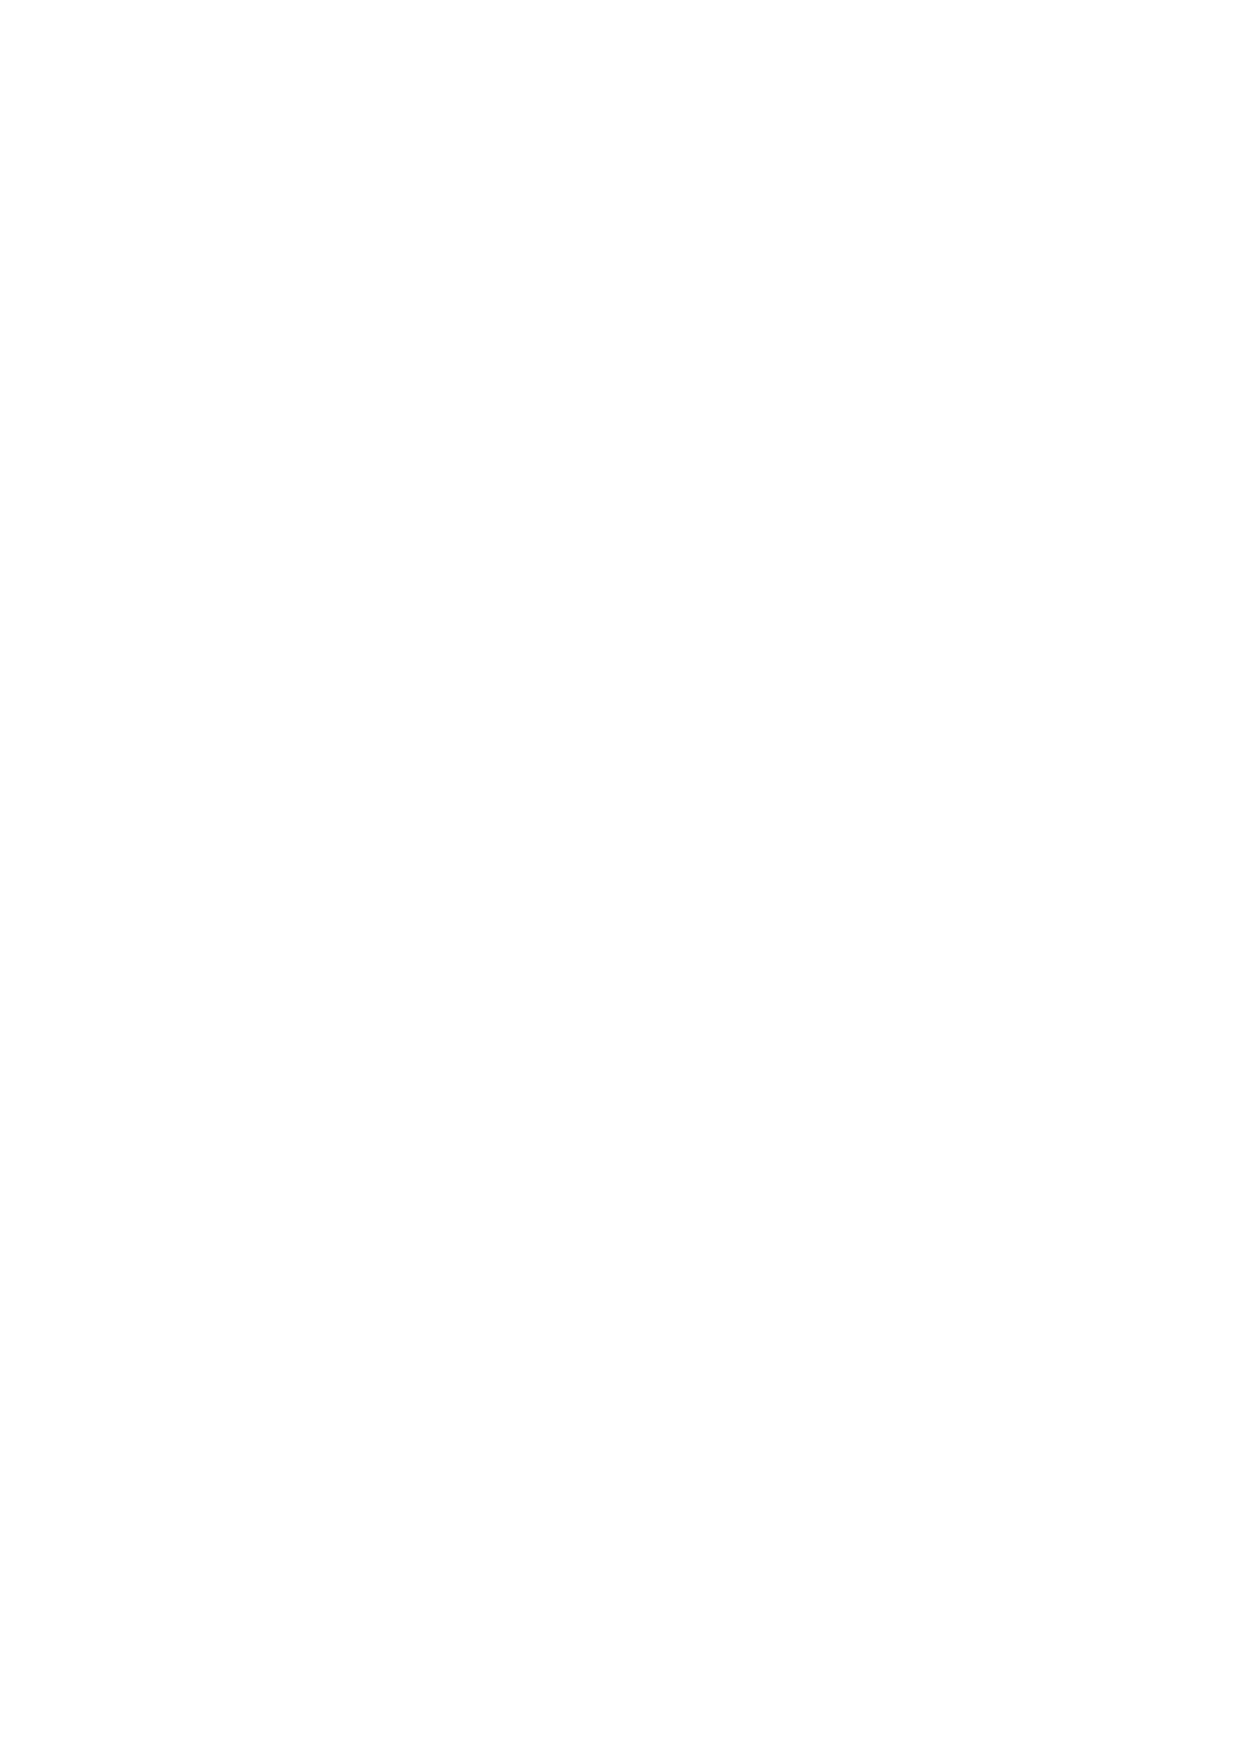
\includegraphics [scale=1]{jtr29}
		\caption{Liénard system.}
		\label{fig:2.9}
	\end{figure}

	To make things all clear, let's consider four areas of the plane (I, II, III, IV) in which we examine $ \frac {d} {dt} \left (R ^ {2} \right) $. They are shown in Figure \ref{fig:2.9}, where at the border between I and II we have $y=y_{0}$ and between borders II and III and between III and IV we have $y=-y_{0}$.
	
	Let us start from $ \left (x_ {0}, y_ {0} \right) $ such that $ R = R_ {0} $ is large and $ y = y_{0} $. We enter the area I where $ \dot {R} <0 $. Here the system is close to the line $ \dot {x} = y, $ $ \dot {y} = - x-y + 1 $, and it is easy to estimate that the change $ \Delta _ {I} R $ radius $ R $ in the domain I is the form
	$$
	\Delta _{I}R=-C_{1}R_{0}+O(1),\text{ \ \ }R_{0}\rightarrow \infty ,
	$$
	where $C_{1}>0$ and does not depend on $R_{0}$.
	
	We enter the area II with radius $ R_ {1} \approx (1-C_ {1}) R_ {0}$. This is a large radius and therefore $ x $ is large (because $ y $ is bounded). Here the phase curves satisfy the equation
	$$
	\frac{dx}{dy}=\frac{-y}{x+\ldots }\approx \frac{-y}{R_{1}+o(1)}
	$$
	and we have an estimate
	$$
	-C_{2}<\Delta _{II}R<C_{2}
	$$
	for a fixed $ C_ {2} $ independent of $ R_ {0}. $
	
	Analogously as in area I we get $\Delta _{III}R=-C_{1}R_{2}+O(1)$
	(where $R_{2}=R_{1}+O(1)$) and, analogously as in area I we get $\left\vert \Delta _{IV}R\right\vert <C_{2}$. By summing up these increments we get
	$$
	\Delta R\leq -2C_{1}R_{0}+C_{3}
	$$
	for a fixed $ C_ {3} $ independent of $ R_ {0}$.
	
	Thus, the radius $ R $ decreases and it is now easy to construct the outer edge of the ring $ \mathcal {R} $; just slightly skew the trajectory of the point $(x_0, y_0)$ and join the ends of the segments.
\end{example}

The readers may ask why in the Poincaré-Bendixson theorem the area $ \mathcal {R} $ is a ring; it may be enough to be bounded and simply-connected (i.e. without a hole in the middle). Well, no, and the reason lies in the following theorem.

\begin{theorem}\label{theo:2.21}
	Inside the area bounded by a closed phase curve of a vector field on the plane there is at least one singular point of this field.
\end{theorem}

The proof of this result uses topological methods, more specifically, the concept of index.

\begin{figure}[!ht]
	\centering
	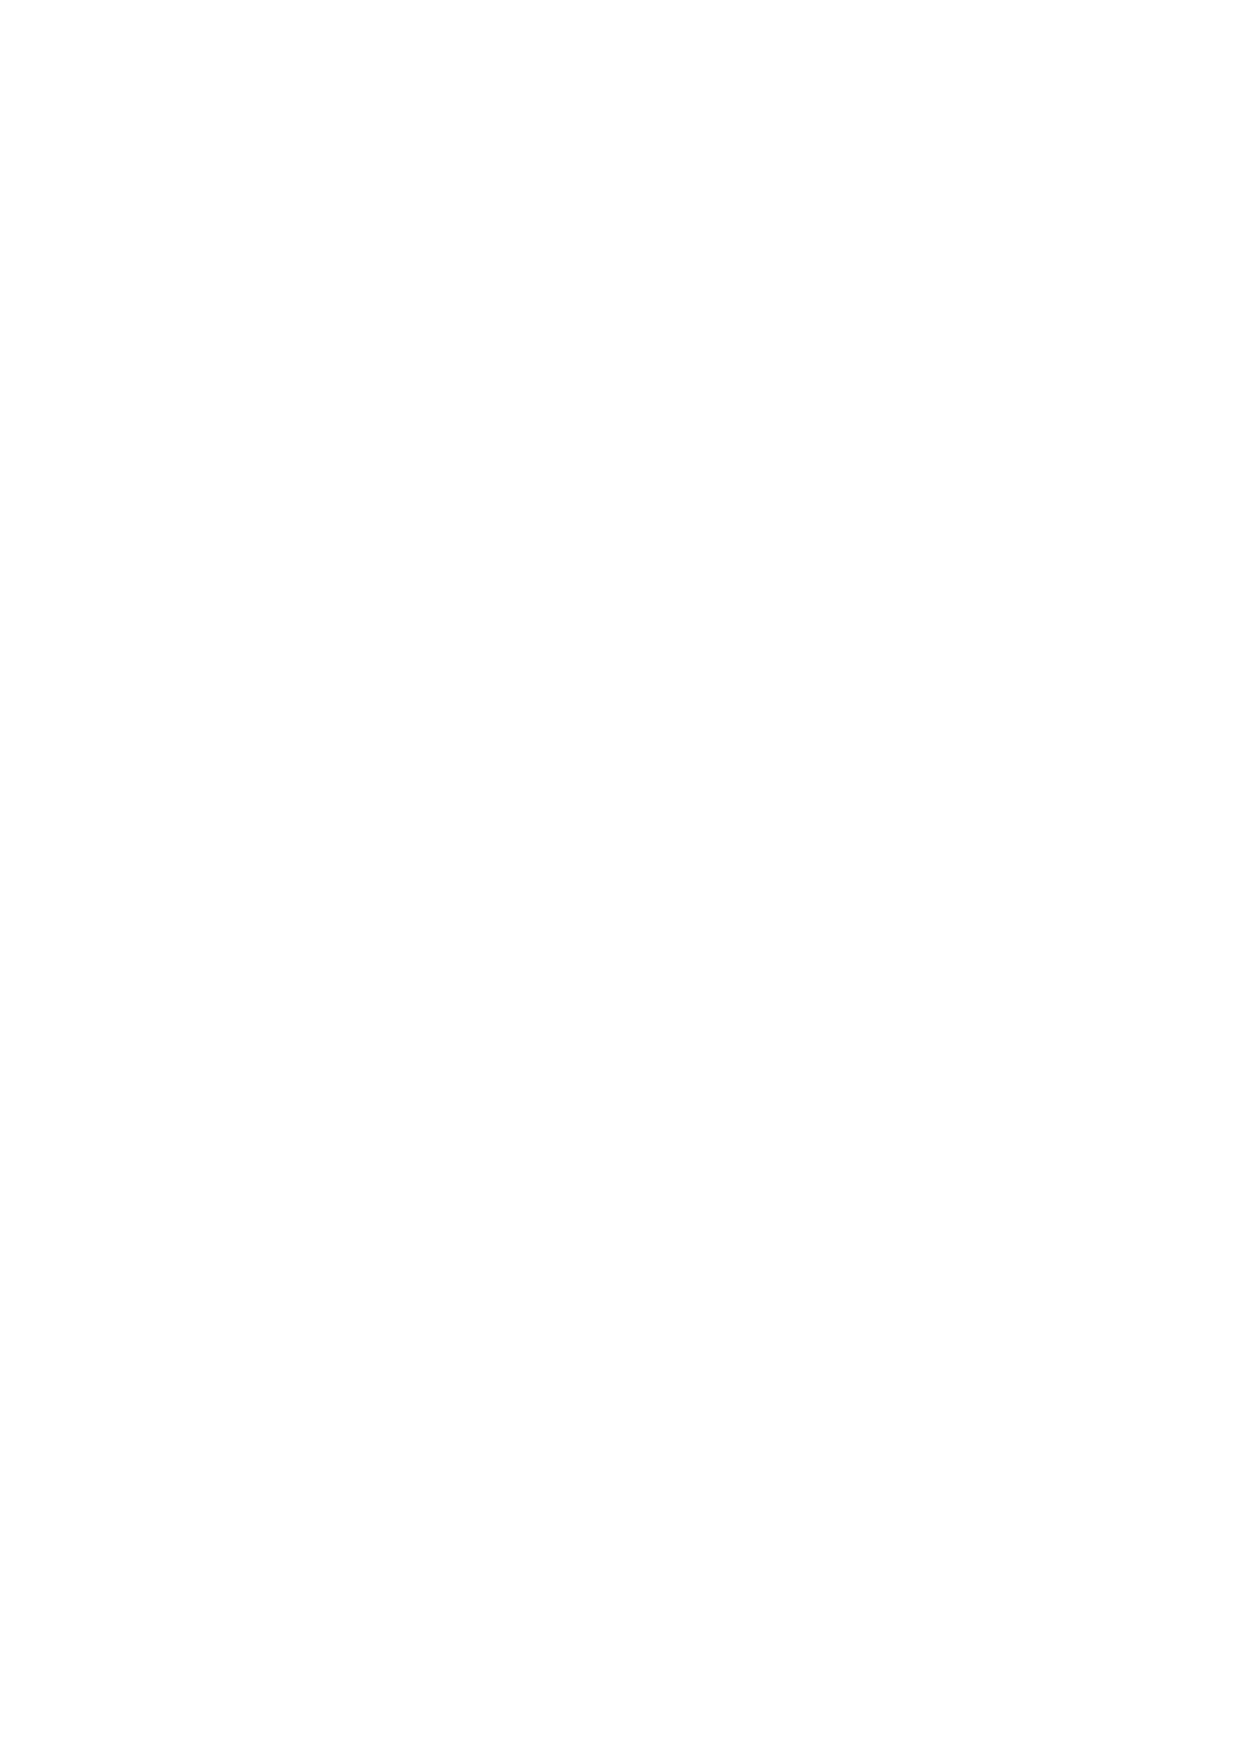
\includegraphics [scale=1.6]{jtr210}
	\caption{Vector field index.}
	\label{fig:2.10}
\end{figure}

\begin{definition}
	Let $ v (x) $ be a vector field in $ \mathbb {R} ^ {2} $ and let $ C \subset \mathbb {R} ^ {2} $ be an oriented curve such that
	\begin{equation}
		\label{2.12}
		v|_{C}\not=0.
	\end{equation}
	The \textbf{index  $i_{C}v$ of the field $v$ along the curve $ C $} is the number of rotations of the vector $ v |_{C} $.
	
	If $ x_ {0} $ is an isolated singular point of field $ v $, then the \textbf{index $ i_ {x_ {0}} v $ of field $ v $ in $ x_ {0} $} is called the index $ i_ {C (x_ {0}, \varepsilon)} v $ of the field $ v $ along the circle $ C (x_ {0}, \varepsilon) $ around $ x_{0} $ with sufficiently small radius $ \varepsilon $ (and counter-clockwise, i.e., positively).\footnote{An index of an isolated singular point $ x_ {0} $ of the vector field $ v (x) $ is generalized to the case of $ \mathbb {R} ^ {n} $. This is the degree of mapping $ x \longmapsto v (x)/ \left \vert v (x) \right \vert $ from the small sphere around $ x_ {0} $ to $ \mathbb {S} ^ {n-1}$.}
\end{definition}

\begin{example}
	For the field $v=x\partial _{x}+y\partial _{y}$ we have $i_{(0,0)}v=1$, for the field $v=x\partial _{x}-y\partial _{y}$ we have $i_{(0,0)}v=-1$ and for the field $v=x^{2}\partial _{x} - y\partial _{y}$ we have $i_{(0,0)}v=0$, see Figure \ref{fig:2.10} (Tasks 2.56 and 2.57).
\end{example}

\begin{proposition}
	For the positively oriented curve $ C $ we have
	$$
	i_{C}v=\sum i_{x_{j}}v,
	$$
	where the summation runs after the singular points within a region bounded by the $ C $ curve.
	
	\begin{proof}
		Let us assume that the mapping
		$$
		\left( v,C\right) \longmapsto i_{C}v
		$$
		is a continuous function over the pair $\left( \text{vector field, curve}\right) $ satisfying condition \eqref{2.12}. Since the set of values of this function are integers, the index is locally constant. In particular, it does not depend on the deformation of the field and the deformation of the curve (see \eqref{2.12}); this justifies the definition of the index in point.
		
		\begin{figure}[!ht]
			\centering
			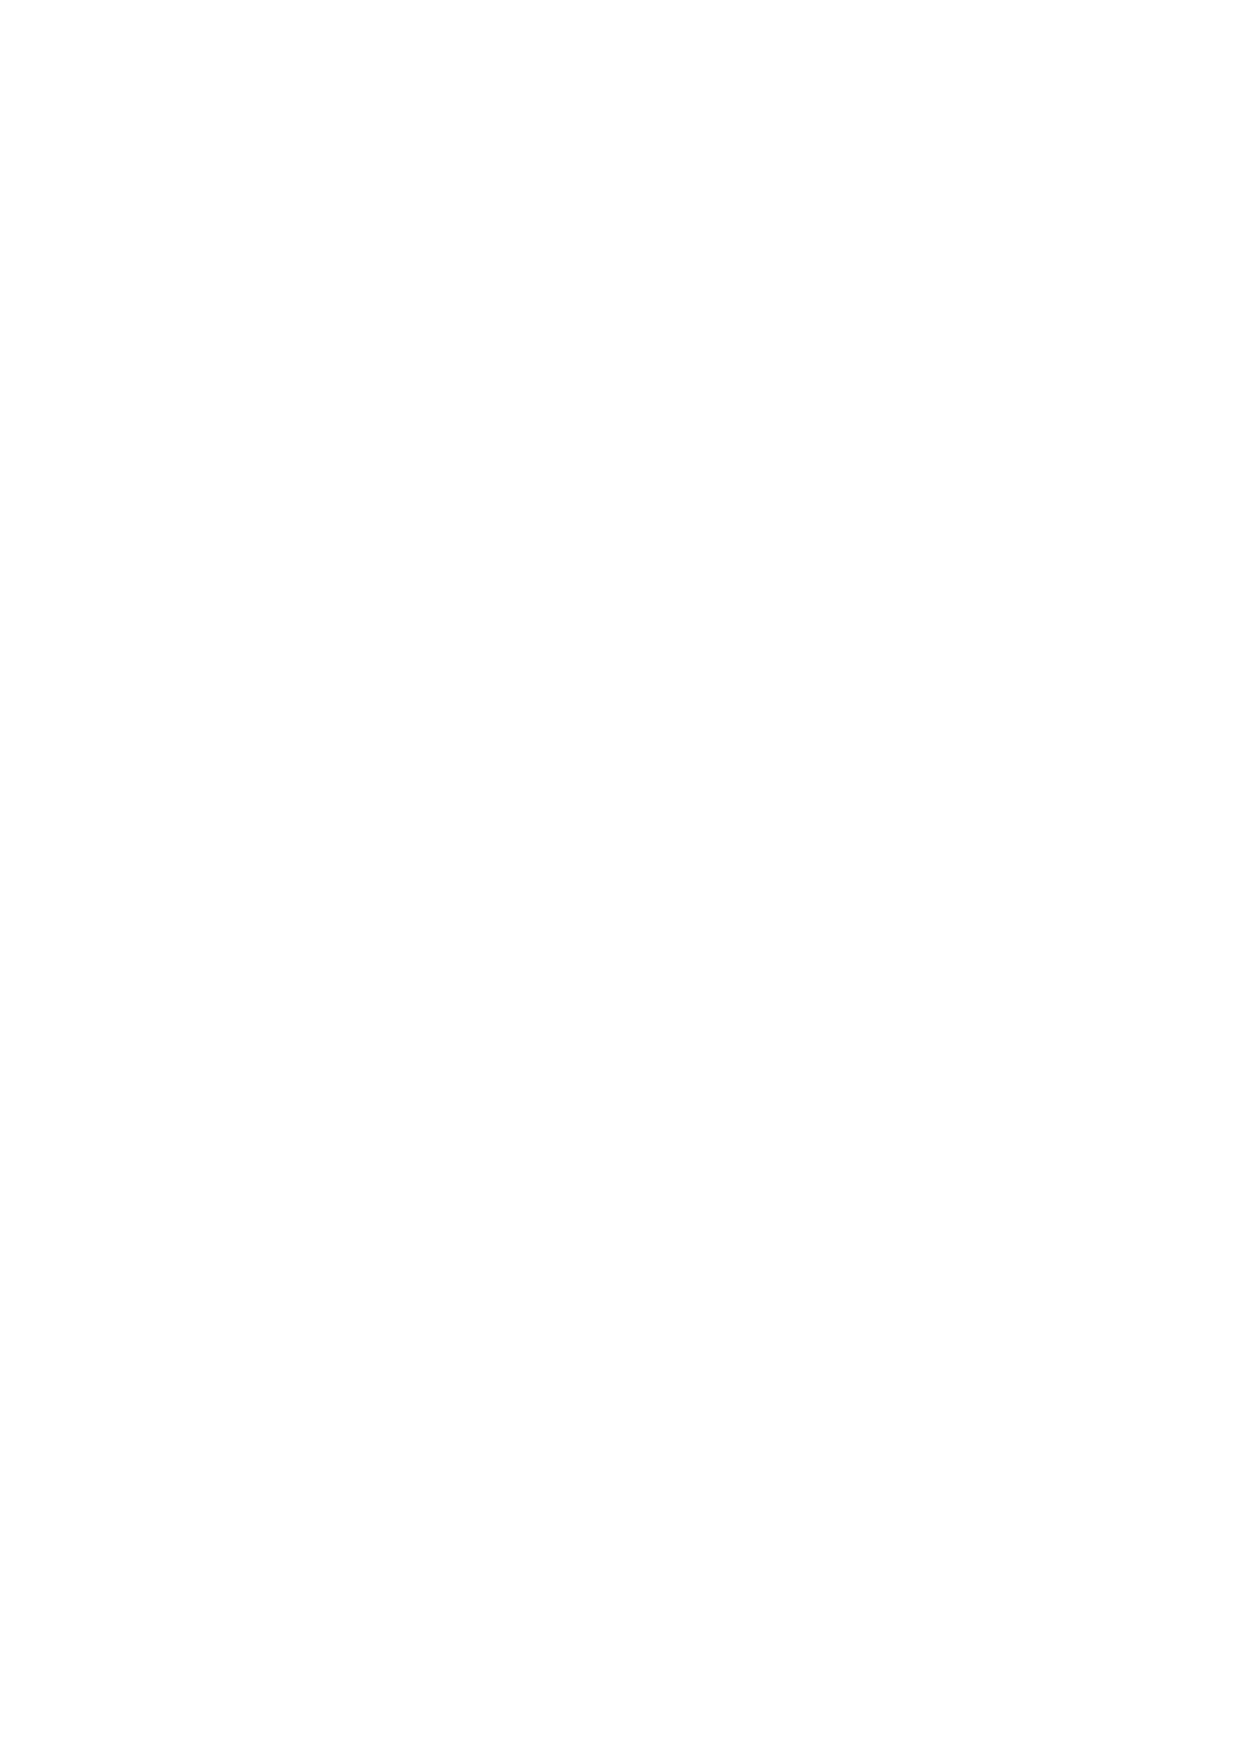
\includegraphics [scale=1.2]{jtr211}
			\caption{Homotopy equivalent curves.}
			\label{fig:2.11}
		\end{figure}
		We can deform the curve to the $ C ^ {\prime}$ curve that is composed of the loops around the equilibrium points $ x_ {j} $ and the system of segments that join these points to the base point. Since the field rotation along the stretches will be in pairs, $ i_ {C_ {1}} v $ is equal to the sum of the field turns around the singular points (see Figure \ref{fig:2.11}).
	\end{proof}
\end{proposition}

\begin{lemma}
	If $ C $ is a closed phase curve of the field $ v $, then $ i_ {C} v =  1$.
	\begin{proof}
		By using the invariant of the index with respect to deformation (see \eqref{2.12}) we can deform the curve and the field to get $ C = \left \{x ^ {2} + y ^ {2} = 1 \right \} $ (with positive or negative orientation) and $ v $ will be tangent to that curve. It is easy to see that the angle of the vector $ v (x, y) $ to $ C $ is `delayed' or `accelerated' in relation to the angle of the point $ \left (x, y \right) $ on $ \pi / 2 $.
	\end{proof}
\end{lemma}

The following corollary implies the Theorem \ref{theo:2.21}.

\begin{corollary}
	If $ \gamma \subset \mathbb {R} ^ {2} $ is a closed phase curve of $ v (x) $, then
	$$
	\sum i_{x_{j}}v=1,
	$$
	where the summation runs over the singular points of the field within the area enclosed by the $ \gamma $ curve.
\end{corollary}

\section{Dulac's criterion}

Let's consider the vector field $ v (x) $, $ x \in \mathbb {R} ^ {2} $, with the closed phase curve $ \gamma $, i.e., the periodic trajectory $ x = \varphi _ {0} (t) $ of period $ T $. Let us consider the section $ S $ (perpendicular to $ \gamma $ at $ x_ {0}$) and the corresponding Poincaré return map $ f: S \longmapsto S $. By identifying $S$ with $\left( \mathbb{R}, 0\right) $ we have
$$
f(z)=\lambda z+O(z^{2}),\text{ \ \ }\lambda >0.
$$

\begin{definition}\label{def:2.27}
	The number $\mu =\ln \lambda $ is called the \textbf{characteristic exponent} of the periodic orbit $ \gamma $. (Task 2.59).
\end{definition}

\begin{remark}
	If $\mu <0$, then $\gamma$ is asymptotically stable (or attracting), whereas if $\mu >0$, then $\gamma$ is repelling.
\end{remark}

\begin{theorem}\emph{(Dulac).}
	We have
	$$
	\mu =\int_{0}^{T}\emph{div\,}v(\varphi _{0}(t)))dt,
	$$
	where $\emph{div\,}v(x)$ denotes the divergence of the vector field $ v (x) $ (see formula \eqref{6.29} below).
	\begin{proof}
		Let's consider the equation in variations with respect to the initial conditions of the solutions $\varphi
		_{0}(t) $%
		$$
		\dot{y}=A(t)y,\text{ \ \ \ }A(t)=\frac{\partial v}{\partial x}(\varphi
		_{0}(t))
		$$
		(see formula \eqref{6.13}). Let us choose two initial conditions for this equation: $ y (0) = y_ {1} $, as a unit vector tangent to $ \gamma $ in $ x_ {0} $, and $ y (0) = y_ {2}$ as a unit vector perpendicular to $ \gamma $ in $ x_ {0} $. One corresponds to two types of initial condition disturbance $ x (0) = x_ {0} $ for the equation $ \dot {x} = v (x)$: $x (0) = x_ {0} + \varepsilon y_ {1} $ and $ x (0) = x_ {0} + \varepsilon y_ {2} $.
		
		\begin{figure}[!ht]
			\centering
			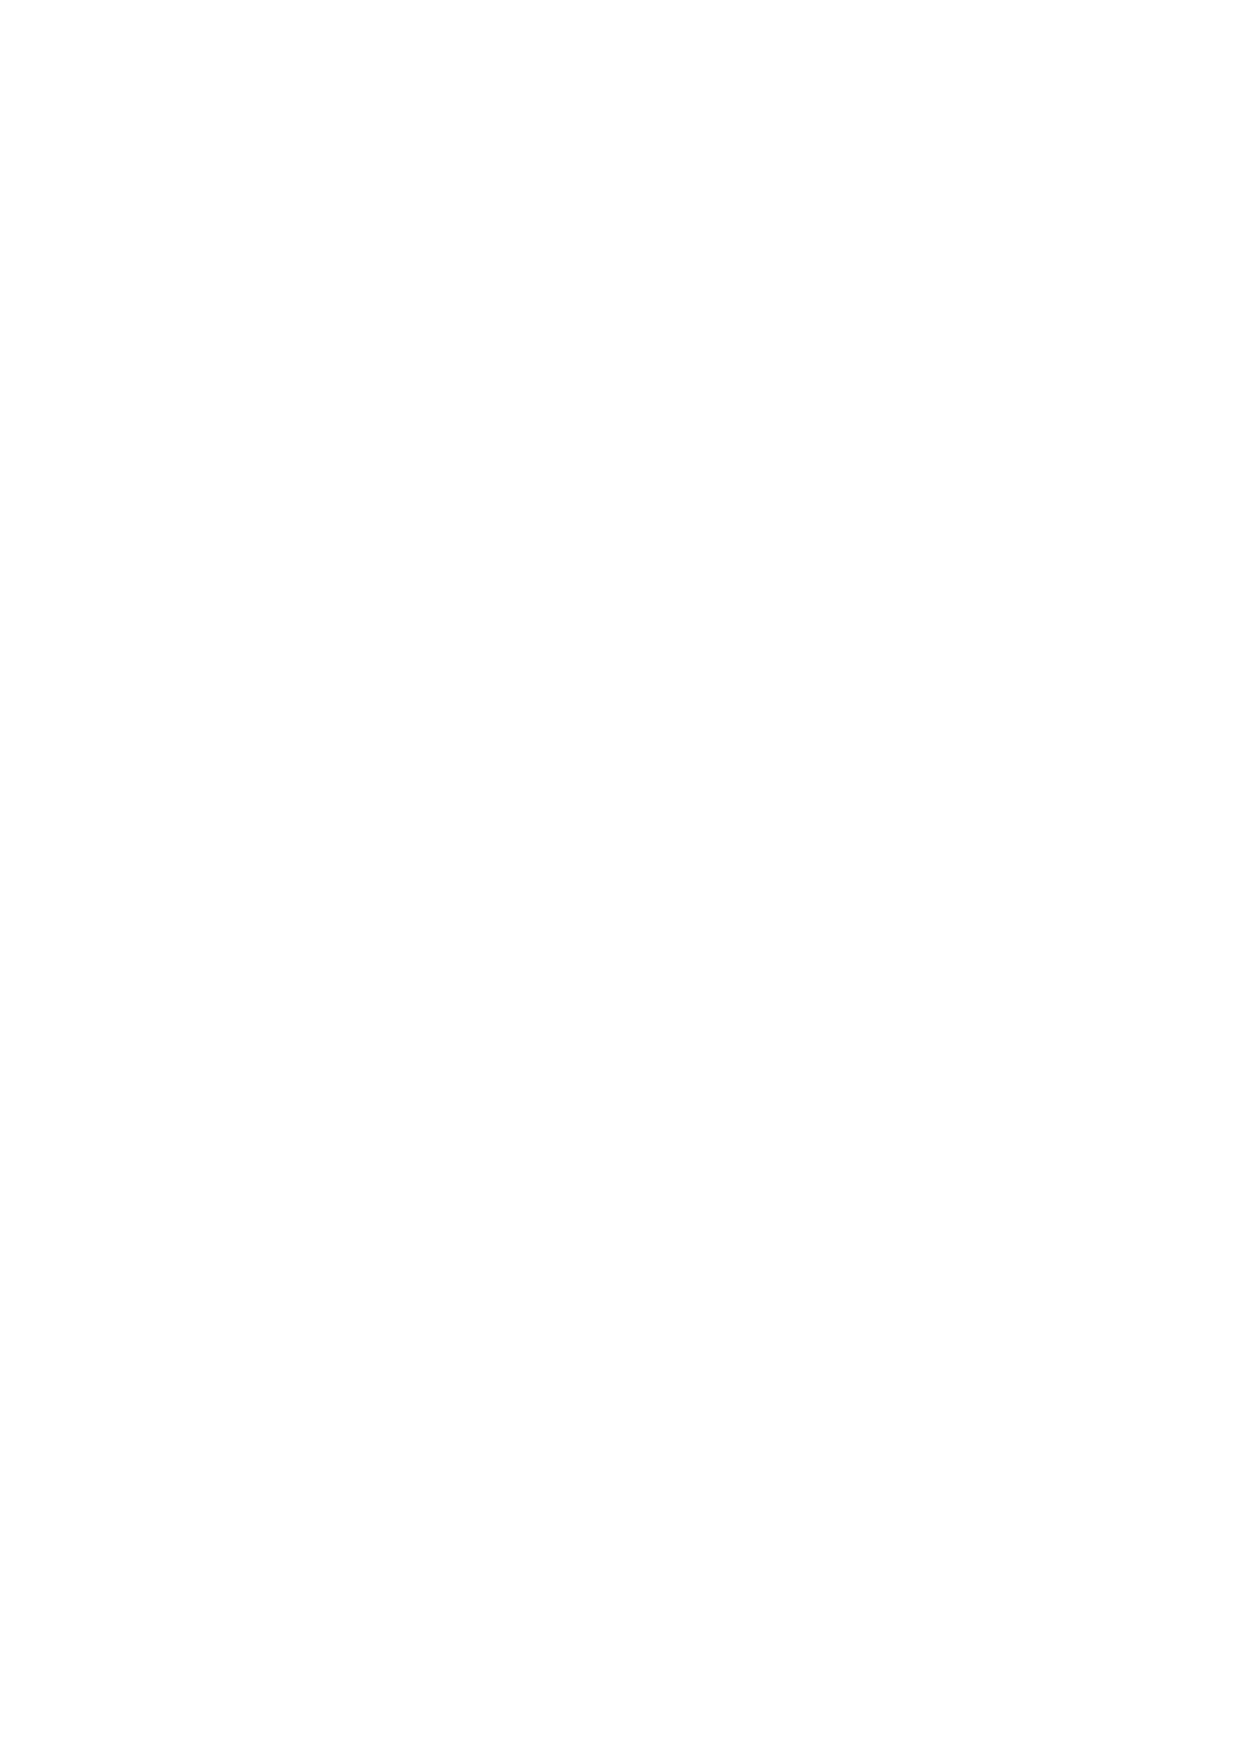
\includegraphics [scale=1]{jtr212}
			\caption{Dulac's theorem.}
			\label{fig:2.12}
		\end{figure}
	
		According to the formula \eqref{6.28}, solutions $y=\psi _{1}(t)$ and $y=\psi _{2}(t)$ satisfying the above initial conditions extend the parallelograms, whose field is equal to the Wronskian $W(t)=\det \left( \psi _{1}(t),\psi _{2}(t)\right) $ solutions. For $t=T$ we have $\psi _{1}(T)=\psi _{1}(0)=y_{1}$, because $x=\varphi _{0}(t)+\varepsilon
		\psi _{1}(t)+O(\varepsilon ^{2})$ actually represents the periodic solution $ \varphi _{0} (t) $ with a slightly shifted starting point (at $ \gamma$). However $ \Psi _ {2} (T) $ is a vector associated with the solution $ x = \varphi _ {0} (t) + \varepsilon \psi_ {2} (t) + O (\varepsilon ^ {3} $ for $ t = T $, which does not even need to hit $S$ (see Figure \ref{fig:2.12}). But the projection $\varepsilon (\psi
		_{2}(T),y_{2})y_{2}$ of the vector $\varepsilon \psi _{2}(T)$ on $ S $ has a natural interpretation of $ f (\varepsilon y_ {1}) + O (\varepsilon ^ {2}) $, where $ f $ is the return map.
		
		Let's now notice that the parallelogram is spread by the vectors $ \psi _ {1} (T) = y_ {1} $ and $ \psi _ {2} (T) $ has the same field $ W (T) $ as the length of the vector projection of $ \psi _ {2} (T) $ on $ S $. This means that
		$$
		f^{\prime }(0)=W(T).
		$$
		But Theorem \ref{theo:6.23}, or $\dot{W}=\textrm{tr}A(t)\cdot W$ with $\textrm{tr}%
		A(t)=\textrm{div}\,v(\varphi _{0}(t))$, allows us to calculate $ W $. Since $ W (0) = 1 $, then we have $ W (T) = \exp \int_ {0} ^ {T} \textrm {tr} A (t) dt $.
	\end{proof}
\end{theorem}

Dulac's theorem turns out to be useful in showing the lack of limit cycles for certain vector fields. We will illustrate this in the following example.

\begin{example} (Jouanolou system).
	It has the following form	
	\begin{figure}[!ht]
		\centering
		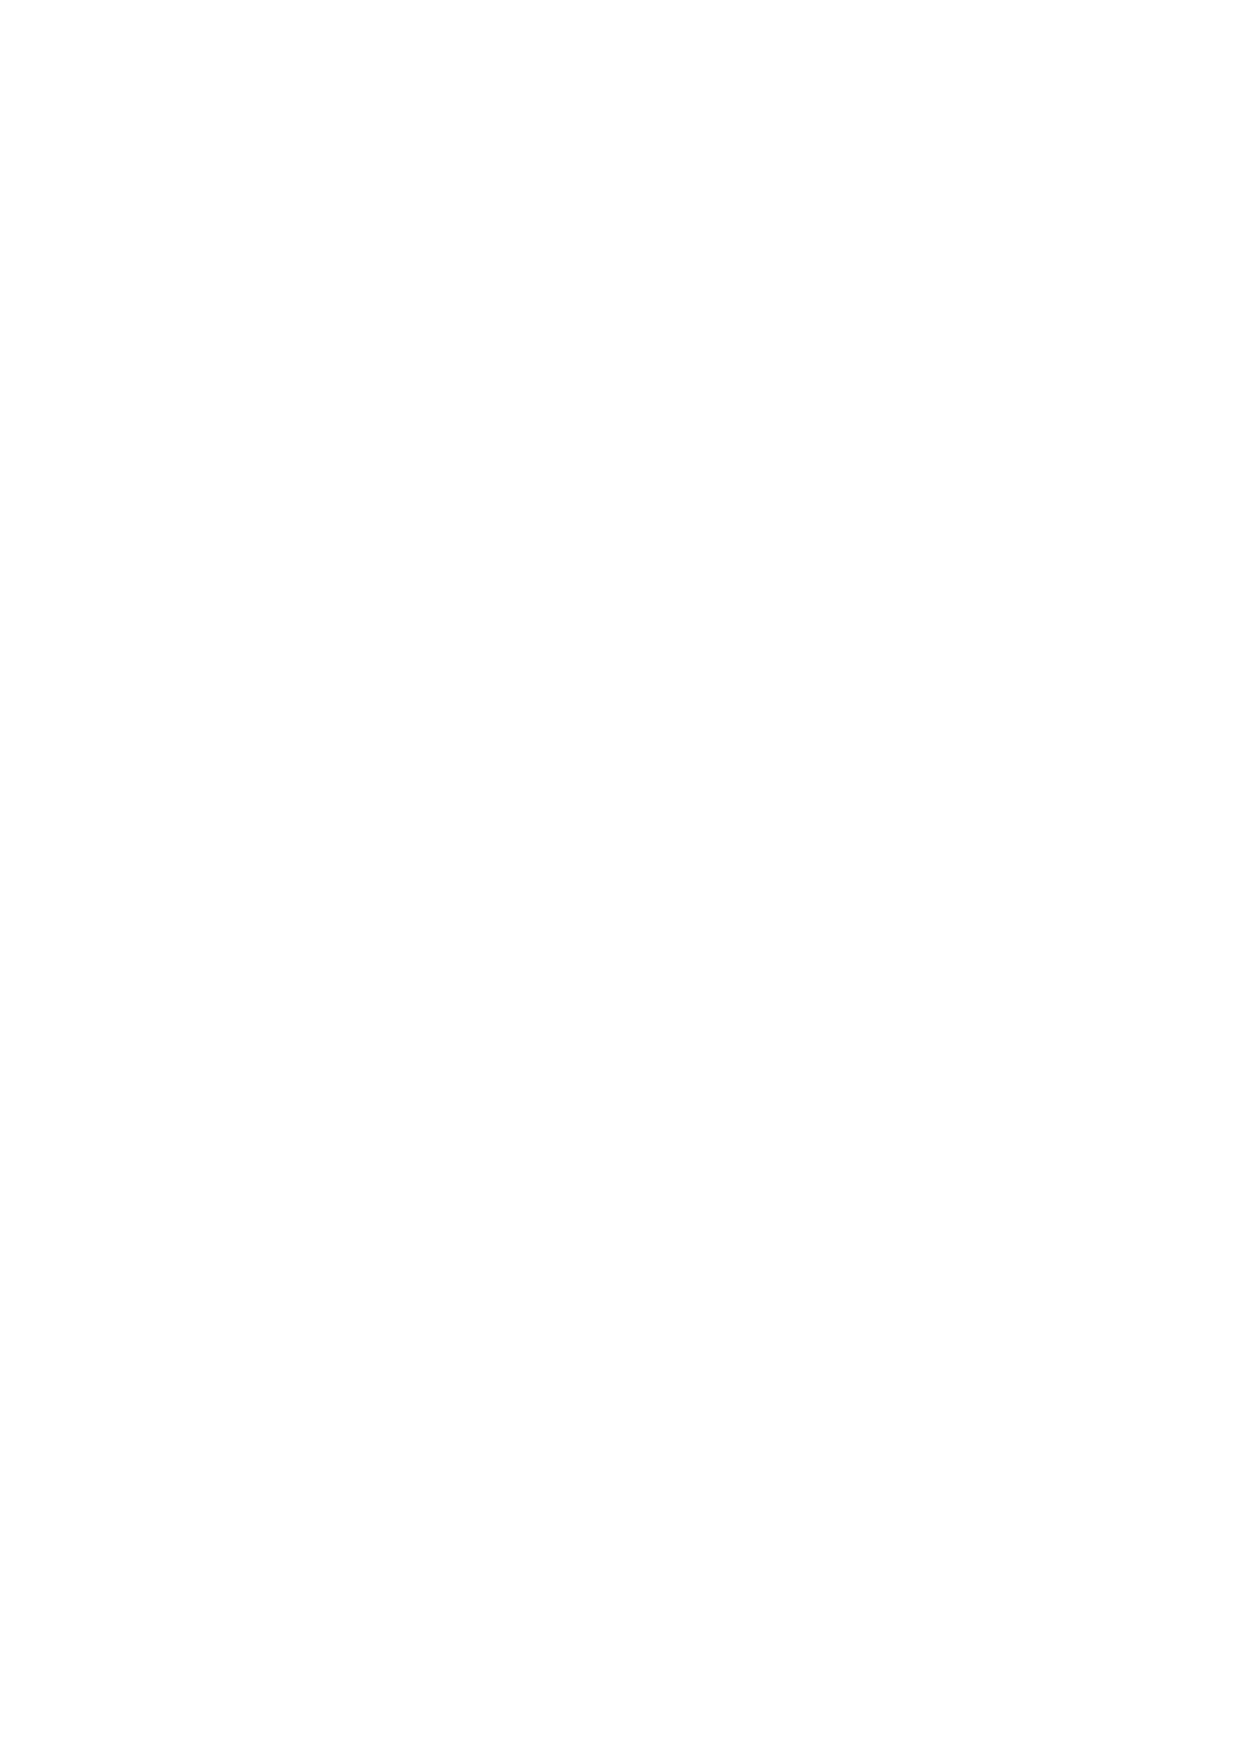
\includegraphics [scale=1.3]{jtr213}
		\caption{Jouanolou system.}
		\label{fig:2.13}
	\end{figure}
	$$
	\dot{x}=y^{s}-x^{s+1},\text{ \ \ }\dot{y}=1-yx^{s}.
	$$
	According to Theorem \ref{theo:2.21}, every limit cycle of this field should surround at least one singular point. Equations of singular points are $y=x^{-s}$ and $\left( x^{-s}\right) ^{s}=x^{s+1}$, which leads to $ x ^ {s ^ {2} + s + 1} = 1$. So there is only one (real) equilibrium point $ x = y = 1. $
	
	The linear part of the system at this point is given by the matrix
	$$
	\left(
	\begin{array}{cc}
	-s-1 & s \\
	-s & -1%
	\end{array}%
	\right)
	$$
	with the characteristic equation $\lambda ^{2}+(s+2)\lambda
	+(s^{2}+s+1)=0. $ So the point $ \left (1,1 \right) $ is a stable focus.
	
	Let us assume that $ \gamma $ is the limit cycle around $ \left (1,1 \right) $ and closest to that point (all limit cycles form a `nest' around $ (1,1) $). It is easy to see that $ \gamma $ must be unstable (at least from the inside).
	
	On the other hand, the divergence of the Jouanolou field is
	$$
	\textrm{div}=-(s+2)x^{s}.
	$$
	We can see that if $ s $ is even, then $\textrm {div} <0 $ (for almost all points of the phase curve) and Dulac's theorem implies that the characteristic exponent of $ \gamma $ is negative (in contradiction with the instability of $ \gamma$).
	
	If $ s $ is odd then this argument also works, but first we need to show that $ \gamma $ must lie in the first quadrant, see Figure \ref{fig:2.13} (Task 2.60).
\end{example}

Dulac's theorem has other uses.

\begin{definition}
	Function $\Phi :\Omega \longmapsto \mathbb{R}_{+}$, $\Omega \subset \mathbb{R}^{2}$, is called the \textbf{Dulac function} for the vector field $v$, if $\textrm{div}\,\left( \Phi v\right) $ has a fixed sign in the domain $\Omega$.
\end{definition}

\begin{theorem}\label{theo:2.32}
	If there exists a Dulac function $\Phi $ in the $\Omega$ region  for the vector field $v$, then every limit cycle lying in $\Omega $ is stable, when $\emph{div}\left( \Phi v\right) <0$ (respectively unstable, when $\emph{div}\left( \Phi v\right) >0$).
	\begin{proof}
		Multiplying the vector field by positive functions does not change the phase portrait of this field. Only the speed of the point (i.e. the solution) changes along the phase curve.
	\end{proof}
\end{theorem}

\begin{remark}
	In Theorem \ref{theo:2.32} let the inequalities $\textrm{div}\left( \Phi v\right) \leq 0$ or $\textrm{div}\left( \Phi v\right) \geq 0$ be blurred. But then we have to exclude the possibility that a possible cycle is completely contained in the $\textrm{div}\,\left( \Phi v\right) =0$ curve.
\end{remark}

\begin{example}(Generalized Lotka-Volterra system).
	This is a system that describes the changing population of predators and preys (such as wolves and rabbits)
	
	\begin{figure}[!ht]
		\centering
		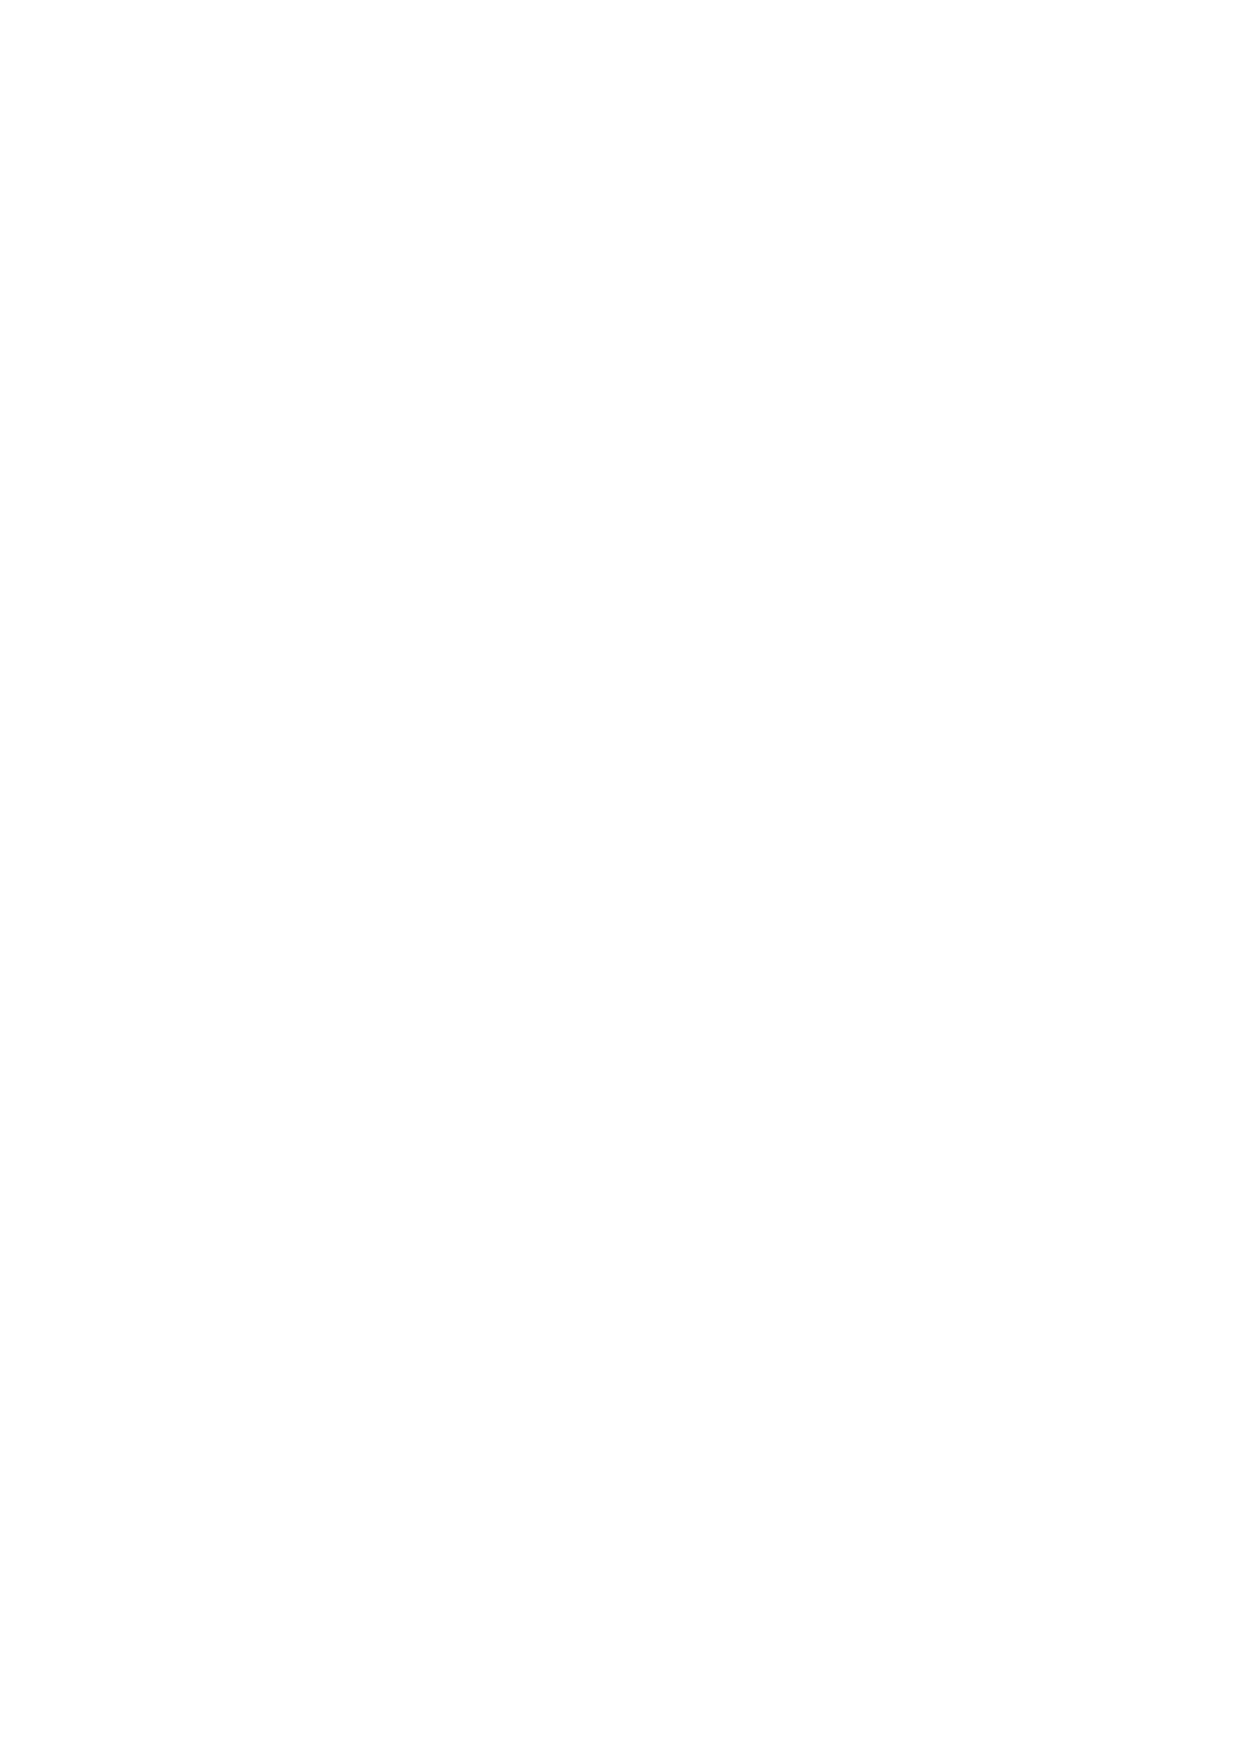
\includegraphics [scale=1.3]{jtr214}
		\caption{Lotka-Volterra system.}
		\label{fig:2.14}
	\end{figure}
	$$
	\dot{x}=x\left[ Ay-B(1-x-y)\right] ,\text{ \ \ }\dot{y}=y\left[ C(1-x-y)-Dx%
	\right]
	$$
	(with $ ABCD \not = 0 $) in the area $ x, y> 0 $. The equations $ Ay = B (1-x-y) $ and $ C (1-x-y) = Dx $ define the singular point $\left( x_{0},y_{0}\right) ,$ which we assume that lies in the first quadrant and that the determinant of the linear part of the matrix in $\left( x_{0},y_{0}\right) $ is positive (only then the index of the field in $\left( x_{0},y_{0}\right) $ is $ 1 $ and there is a chance for the limit cycle). Assume that:
	
	\textit{if $A = D$ then we have a center in $(x_0, y_0)$ and if $A\not=D$ there is no periodic solution.}\\
	To confirm this, consider the following candidate for the Dulac function
	$$
	\Phi =x^{C/A-1}y^{B/D-1}.
	$$
	We check (from $ z = 1-x-y $):	
	$$
	\begin{array}{ll}
	\text{div} \left( \Phi v\right)& =  \frac{\partial }{\partial x}x^{C/A}%
	\left[ Ay-B(1-x-y)\right] y^{B/D-1}
	+\frac{\partial }{\partial y}y^{B/D}\left[ C(1-x-y)-Dx\right] x^{C/A-1}\\
	& =  x^{C/A-1}y^{B/D-1}\left\{ \frac{C}{A}\left[ Ay-Bz\right] +Bx+\frac{B}{D}%
	\left[ Cz-Dx\right] -Cy\right\}\\
	& =  \frac{BC}{AD}(A-D)x^{C/A-1}y^{B/D-1}z.
	\end{array}
	$$
	If $A=D$, then the field $\Phi v$ is Hamiltonian and has a first integral (Figure \ref{fig:2.14}).
	
	If $A-D\not=0,$ then $\Phi $ is the Dulac function in the area $z>0$ or in the area $z<0$. But the identity
	$$
	\dot{z}|_{z=0}=(D-A)x(1-x)\not=0
	$$
	(at $ A-D \not = 0) $ implies that the possible limit cycle can not pass through the segment $x+y=1,$ $x,y>0$. Further reasoning is the same as in the example of the Jouanolou system.
\end{example}

\begin{example}\label{example:2.35}(Van der Pol equation). 
	This is the following equation
	$$
	\dot{x}=y,\text{ \ \ }\dot{y}=-x-a(x^{2}-1)y,\text{ \ \ }a>0;
	$$
	special case of the Liénard system. It appears in electrical engineering, for a system consisting of a capacitor of capacity $C$, a coil of inductance $L$ and a certain nonlinear element (type of diode) replacing a resistor. In case of $LCR$ system (coil, capacitor, resistor) the equation of potential differences gives the equation $L\ddot{I}+R\dot{I}+I/C=0$ for the current of $ I $ in the circuit; in our case, the member $\frac{d}{dt}\left( RI\right) $ is replaced by the member $\frac{d}{dt}\left[ R\left( I^{3}/3-I\right) \right]$, i.e.,
	$$
	L\ddot{I}+R(I^{2}-1)\dot{I}+I/C=0;
	$$
	is the original \textbf {Van der Pol equation}. After replacing $t\longmapsto \alpha t=\sqrt{CL}t$ and substituting $x = I$ and $y = \dot{ I}$, we obtain the above Van der Pol system with $a=R/\alpha $. For more details, refer to D. Arrowsmith and K. Place's book \cite{ArPl}.
	
	We will prove that:
	\begin{figure}[!ht]
		\centering
		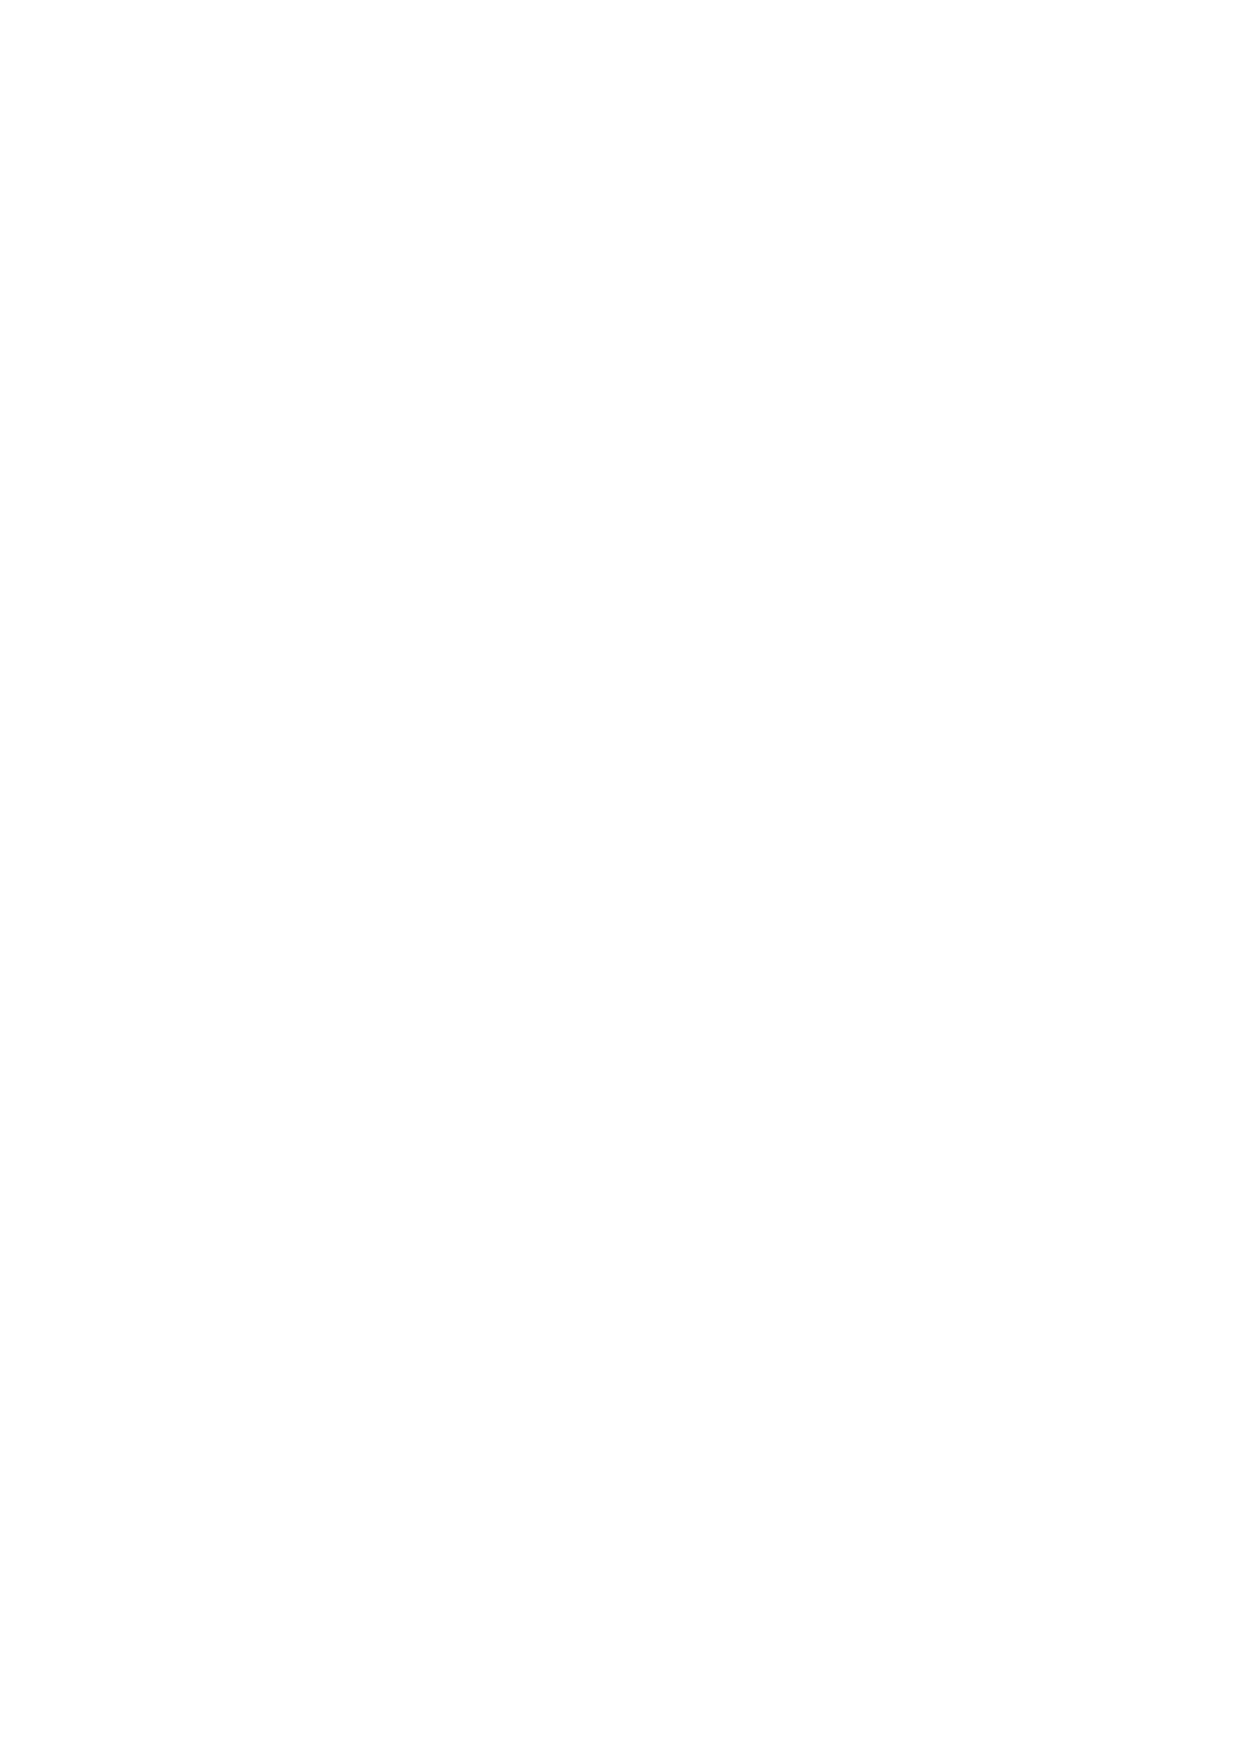
\includegraphics [scale=1]{jtr215}
		\caption{Function $g(z)$.}
		\label{fig:2.15}
	\end{figure}

	\textit{Van der Pol system has exactly one stable limit cycle.}
	
	First, let us note that $(0, 0)$ is the only singular point with the linearization matrix $\left(
	\begin{array}{ll}
	0 & 1 \\
	-1 & a%
	\end{array}%
	\right) ,$ that is, $\textrm{Re}\lambda _{1,2}>0$ and this point is unstable (focus or node).
	
	Let's consider the function
	$$
	\begin{array}{lll}
	f(x,y) &=&y^{2}+a(x^{3}/3-3)y+x^{2}-c \\
	&=&\left[ y+\frac{1}{2}a\left( \frac{x^{3}}{3}-x\right) \right]
	^{2}-g(x^{2})-c \\
	&=&y_{1}^{2}-g(x^{2})-c,
	\end{array}
	$$
	where
	$$
	g(z)=\frac{a^{2}}{36}z^{3}-\frac{a^{2}}{6}z^{2}+\left( \frac{a^{2}}{4}%
	-1\right) z
	$$
	 is constant $c> 0$ and is small enough. We are interested in the curve $f(x,y)=0, $ which in the coordinates $\left( x,y_{1}\right) $ has the form $y_{1}=\pm \sqrt{g(x^{2})+c}$.  From the properties: $g(0)=0$; $g^{\prime }(0)<0 $ for $0<a<2$; $g^{\prime }(0)>0$ for $a>2$; $g^{\prime
	 }(0)=0$ and $g^{\prime \prime }(0)<0$ where $a = 2$, we can reproduce the graph of $g (z)$; it is shown in Figure \ref{fig:2.15}. Hence, the shape of the curve $ f = 0 $ on the plane of the variables $ x, y_ {1} $ (shown in Figure \ref{fig:2.16}). On the plane of variable $ x, y $ this curve is some sense `kicked'. Let us note that the curve $f = 0$ has three components, one of which is the point $(0, 0)$.
 
	 It turns out that the function
	 $$
	 \Phi (x,y)=1/f(x,y)
	 $$
	 is the Dulac function for the Van der Pol system in the domain $f> 0$.
	 
	 Actually, we have
	 $$
	 \textrm{div}\,\left( \frac{1}{f}v\right) =\frac{f\cdot \textrm{div}\,v-\dot{f
	 }}{f^{2}},
	 $$
	 where
	 $$
	 f\cdot \textrm{div}\,v-\dot{f}=-a\left( \frac{2}{3}x^{4}-cx^{2}+c\right)
	 =:M(x)
	 $$
	 and $M(x)<0$ for $0<c<8/3$ (Task 2.61).
	 
	 \begin{figure}[!ht]
	 	\centering
	 	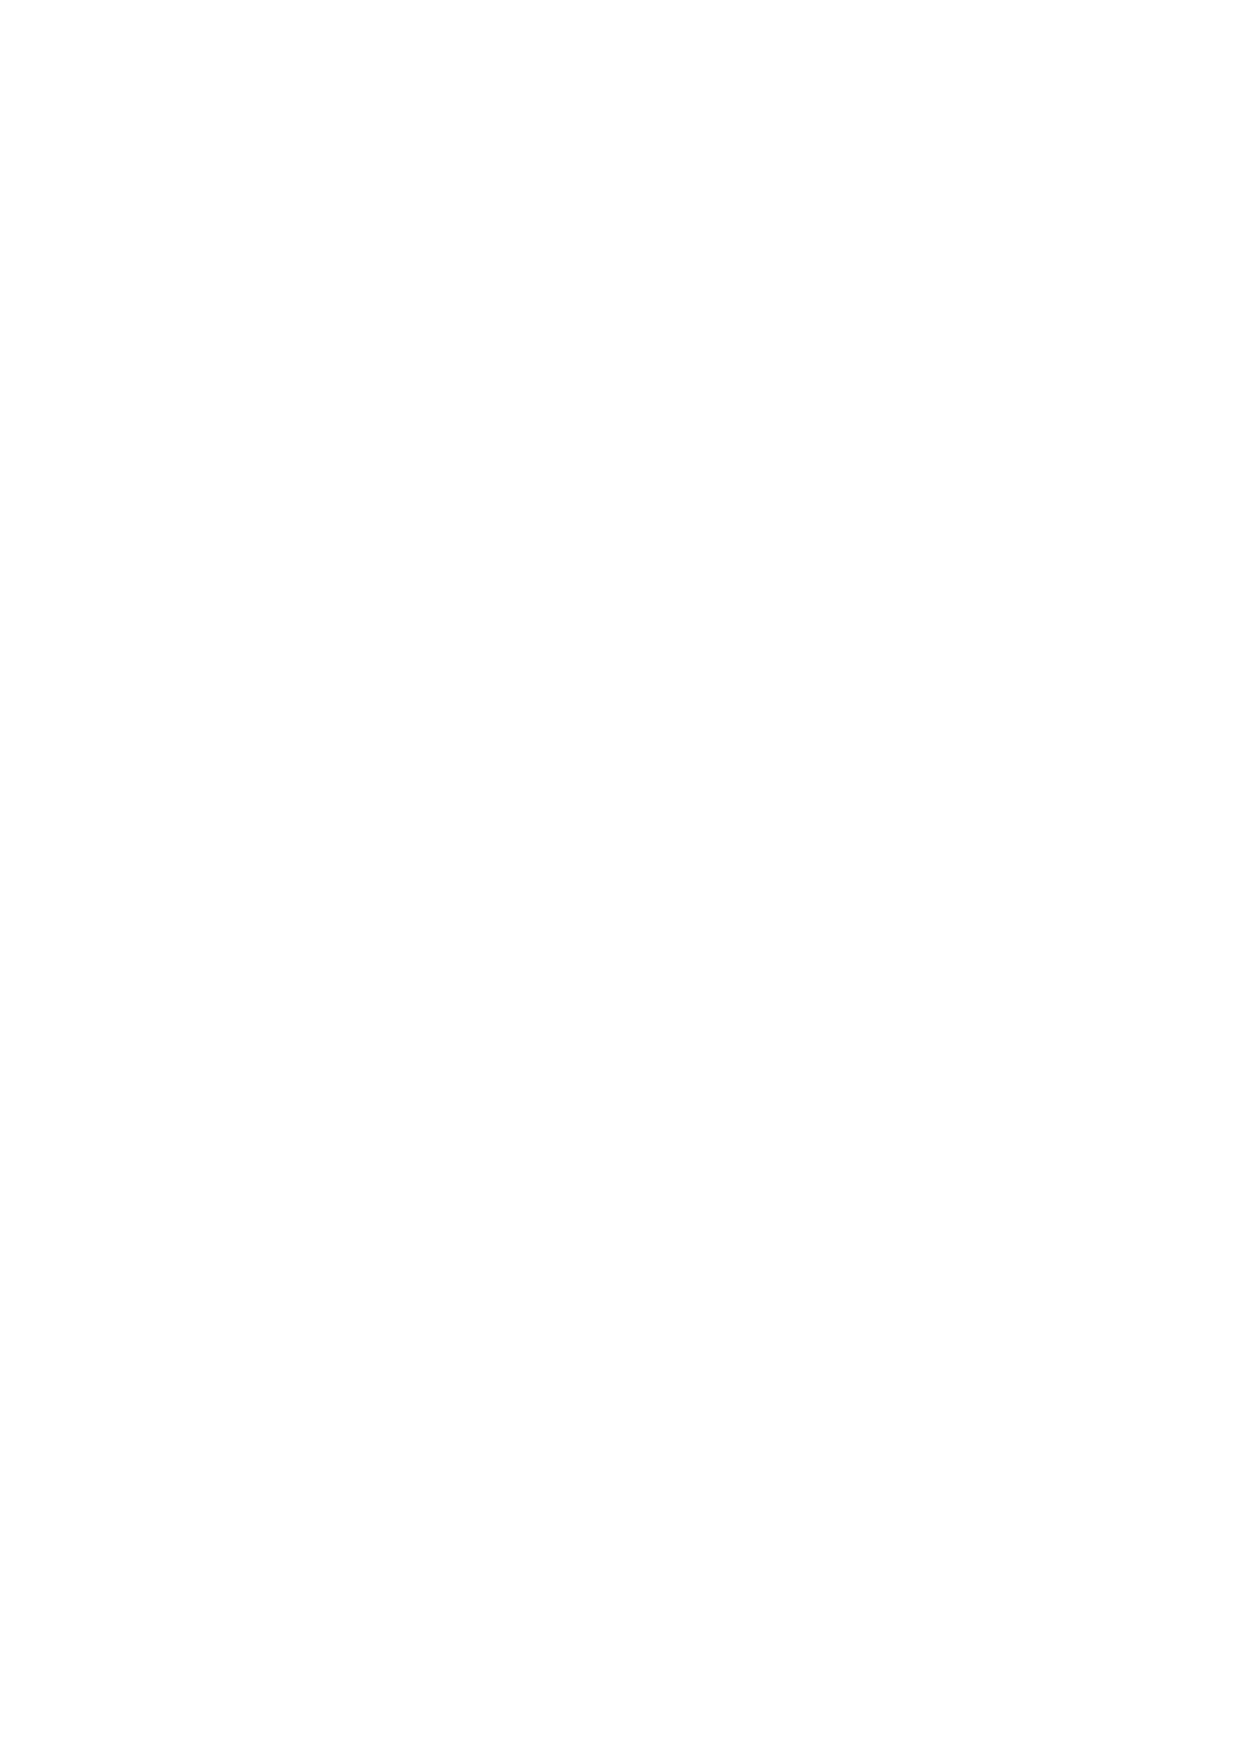
\includegraphics [scale=1]{jtr216}
	 	\caption{Function $f(x,y)$.}
	 	\label{fig:2.16}
	 \end{figure}
 
 	Here we get two applications:
 	\begin{enumerate}[(a)]
 		\item $\dot{f}|_{f=0}>0$, i.e., the vector field is directed into the interior of the area $f> 0$;
 		\item in the area $ f> 0 $, the vector field $\Phi v$ may have at most one limit cycle and stable. Also $v$ can have a unique limit cycle.
 	\end{enumerate}
 
 	It remains to prove that there is a limit cycle in $f> 0$. For this we construct the ring $ \mathcal {R} $ satisfying the assumptions of Poincaré-Bendixson's Theorem. The inner edge of this ring is a small closed component of the curve $f = 0$ around $(0, 0)$. The outer boundary will be composed of unrestricted segments of the curve $f = 0$ and from the `corrected' arcs of the circle  $x^{2}+y^{2}=R^{2}$ for the large radius $R$.
 	
 	From property (a) it follows that on the pieces of the edge in $f = 0$ the field goes to the interior of $\mathcal{R}$. Next, from
 	$$
 	\frac{d}{dt}\left( x^{2}+y^{2}\right) =-2a\left( x^{2}-1\right) y^{2}
 	$$
 	it follows that $ \dot {R} <0 $ is outside the $\left\{ \left\vert x\right\vert \leq 1\right\}$ band. But in this band we have
 	$$
 	\frac{dy}{dx}=-a(x^{2}-1)-\frac{x}{y}=O(1)+O(1/R),
 	$$
 	i.e., the increment $y$ (and hence the increment $R$) is bounded by a constant independent of $R$. Now it is easy to correct the corresponding pieces of the outer edge of the ring $\mathcal{R}$ so that the field also enters $\mathcal{R}$ (see Example \ref{example:2.20}).
 	
 	The above proof of the uniqueness of the boundary cycle comes from L. Cherkassy from Minsk, Belarus. In Task 4.17 below, we propose another proof of the uniqueness of the boundary cycle in case the parameter $a> 0$ is small.
\end{example}

\section{Drawing phase portraits on the plane} \label{sec:2.4}

\begin{figure}[!ht]
	\centering
	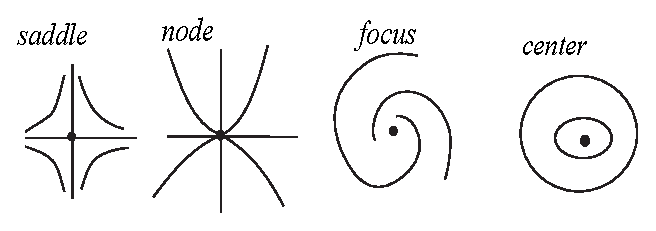
\includegraphics [scale=1.3]{jtr217}
	\caption{Non-degenerate singular points.}
	\label{fig:2.17}
\end{figure}

As already stated in Definition \ref{def:2.1}, the phase portrait of the vector field $v (x)$ on the plane is the split of the plane $\mathbb{R}^{2}$ into the phase curves of that field. The phase portrait elements are: singular points, closed phase curves, separatrix of singular points and behavior on infinity. We will briefly discuss them.

\subsection{Singular points}
They are divided into elementary and non-elementary. The elementary singular points can be subdivided into non-degenerated and degenerate ones.

\begin{definition}
	The equilibrium point $x_0$ of the vector field $v (x)$, $x \in \mathbb{R}^n$, is called \textbf{non-degenerated} if $\det \frac{\partial v}{\partial x}(x_{0})\not=0.$
	
	The equilibrium point $x_0$ of the vector field $v (x)$, $x \in \mathbb{R}^n$, is called \textit{elementary} if at least one of the eigenvalues of the matrix $A=\frac{\partial v}{\partial x}(x_{0})$ is nonzero. In this case, the point $ x_ {0} $ is:
	\begin{itemize}
		\item a \textbf{saddle}, if $\lambda _{1}<0<\lambda _{2}$ for the eigenvalues $\lambda _{1,2}$ of the matrix $A$;
		\item a \textbf{stable node} (respectively an \textbf{unstable node}), if $\lambda _{1},\lambda _{2}<0$ (respectively $\lambda _{1},\lambda _{2}>0$);
		\item a \textbf{stable focus} (respectively \textbf{unstable focus}), if $\lambda _{1,2}\in \mathbb{C}\setminus \mathbb{R}$ and $\textrm{Re}\lambda _{1,2}<0$ (respectively  $\textrm{Re}\lambda _{1,2}>0)$;
		\item a \textbf{saddle-node}, if $\lambda _{1}=0$, $\lambda _{2}\not=0.$
	\end{itemize}
\end{definition}

Local phase portraits surrounded by elementary singular points defined above are shown in Figures \ref{fig:2.17} and \ref{fig:2.18}.

\begin{remark}
	In the case of $\lambda _{1,2}\in i\mathbb{R}\setminus 0$, i.e., purely imaginary values, the critical point $x_0$ may be a stable or unstable focus (more precisely, \textbf{weak focus}) or \textbf{center}; see Proposition \ref{prop:2.11} above.
\end{remark}

\begin{remark}
	The concept of saddle-node given above is quite wide. The point is that we can have the following model situations
	\begin{eqnarray}
	\dot{x} &=&x^{2k},\text{ \ \ }\dot{y}=\pm y,  \label{2.13} \\
	\dot{x} &=&\pm x^{2k+1},\text{\ \ \ }\dot{y}=\pm y.  \label{2.14}
	\end{eqnarray}
	In Section \ref{sec:3.3} below, formulas \eqref{2.13} - \eqref{2.14} will be more justified. When $\dot{x}=x^{s}$ and $ s>2$, then the saddle-node is somewhat degenerated; we say that it has \textit{codimension} $s-1$.
	
	From the topological point of view, the local phase portrait does not depend on $ k$. These portraits are shown in Figure \ref{fig:2.18}.
	
	\begin{figure}[!ht]
		\centering
		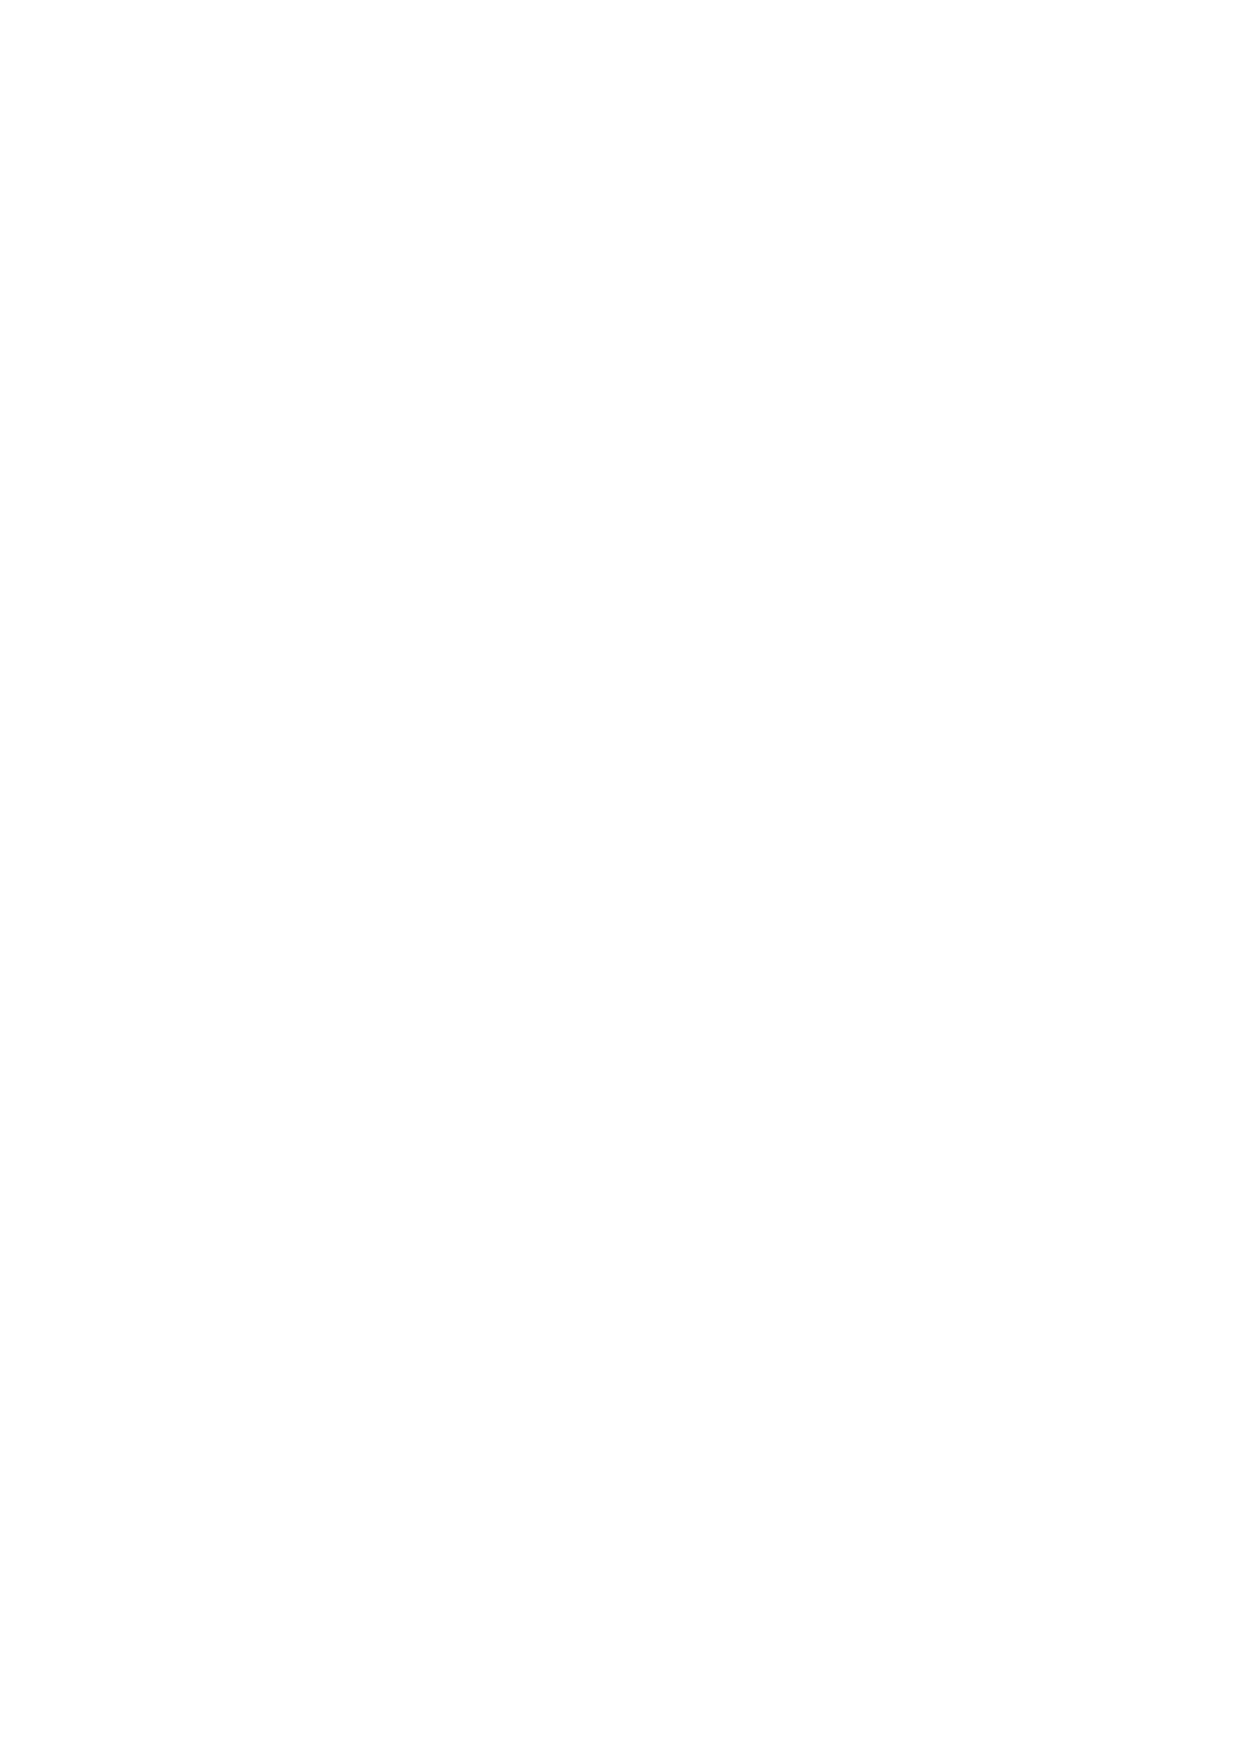
\includegraphics [scale=1]{jtr218}
		\caption{Saddle-node.}
		\label{fig:2.18}
	\end{figure}
\end{remark}

\begin{remark}(Non-elementary singular points).
	Let us remind that here we have $\lambda _{1}=\lambda _{2}=0.$ Unfortunately, there is no satisfactory classification of such singularities. But there is an effective method of researching them. This is the method of \textit{blowing-up singularities} (or solving singularities).
	
	It consists of a simple operation of introducing the polar coordinates $ \left (r, \varphi \right) $ on the plane. So if we have, for example,
	\begin{equation}
	\label{2.15}
	\dot{x}=ax^{2}+bxy+cy^{2}+\ldots ,\text{ \ }\dot{y}=dx^{2}+exy+fy^{2}+\ldots
	,
	\end{equation}
	in the polar variables we get
	\begin{equation}
	\label{2.16}
	\dot{r}=r^{2}\left( P(\varphi )+O(r)\right) ,\text{ \ \ }\dot{\varphi}%
	=r\left( Q(\varphi )+O(r)\right) ,
	\end{equation}
	where
	\begin{eqnarray*}
		P &=&a\cos ^{3}\varphi +(b+d)\cos ^{2}\varphi \sin \varphi +(c+e)\cos
		\varphi \sin \varphi +f\sin ^{3}\varphi , \\
		Q &=&d\cos ^{3}\varphi +(e-a)\cos ^{2}\varphi \sin \varphi +(f-b)\cos
		\varphi \sin \varphi -c\sin ^{3}\varphi .
	\end{eqnarray*}
	Note that the right side of the equation \eqref{2.16} will disappear at $r = 0$. Let's divide these right-hand sides by $r$; in the area $r> 0$, the phase portrait will not change, but the `velocity' of the point along the phase curve will be different, but not zero (it could happen that $Q(\varphi )\equiv 0$, but then we divide by $r^2$). This is so-called orbital equivalence, as described below.
	
	But after this operation we get a vector field on the cylinder $\left\{ \left( r,\varphi \right) \right\} \simeq \mathbb{R}\times \mathbb{S}^{1}$ (for which we have an important part $\left\{ r\geq 0\right\} $), with isolated singular points on the circle $r = 0$. If the coefficients $a,\ldots ,f$ are typical, these singular points are already non-degenerated, i.e., elementary.
	
	Otherwise we repeat the procedure of blowing-up (combined with division) in the neighborhood of each non-elementary singular point $r = 0$, $\varphi =\varphi _{0}$ (with new coordinates $x=\varphi -\varphi _{0}$, $y=r$). It turns out that if the original vector field \eqref{2.15} is analytic, then after the finite number of such blows we get a vector field on a surface $M$ with elementary singular points. (This is a difficult statement, after which I refer to my book \textquotedblleft The monodromy group\textquotedblright\ \cite{Zol2}.)
\end{remark}

\begin{figure}[!ht]
	\centering
	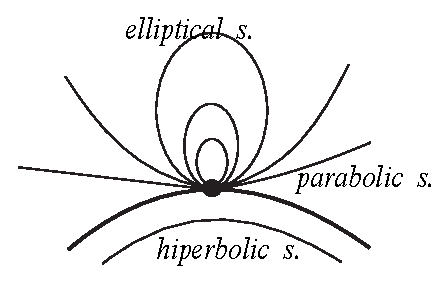
\includegraphics [scale=1.4]{jtr219}
	\caption{Sectors.}
	\label{fig:2.19}
\end{figure}

In the case of non-elementary singular points, its surroundings can be often divided into sectors: \textit{hyperbolic, parabolic and elliptical}. They are illustrated in Figure \ref{fig:2.19}. There is a theory associated with them, which we will not deal with. For interested readers refer to P. Hartman's \cite{Hart}.

\subsection{Closed phase curves}
They correspond to the periodic solutions (and trajectories) and were discussed in detail in the previous section.

\subsection{Separatrix of singular points}
\begin{definition}
	\textbf{Separatrix of a singular point} $x_0$ of the vector field $v (x)$ is how is called the phase curve of that field which `tends' to $x_0$ under a certain limit direction among such curves.
\end{definition}

For example, for the saddles, separatrices there are components of the `perforated' manifolds, stable $ W ^ {s} \setminus x_ {0} $ and unstable $ W ^ {u} \setminus x_ {0} $; in total we have four separatrices.

In the general case, when we divide into hyperbolic, elliptical, and parabolic sectors, separatrices occurs on the edges of hyperbolic sectors.

\begin{remark}
	An important element of the phase portrait of the vector field is the `fate' of the second end of the separatrix $L$.
	
	It can be loaded at another singular point $x_1$, usually in its parabolic sector. But it can also turn into a focus. Particularly is the case where $L$ is a separatrix for both $x_0$ and for $x_1$; we are dealing with the so-called \textit{separatrix connection}.
	
	The other end of the separatrix can also end on the limit cycle.
	
	Particular and useful in the theory of Dynamic Systems is the case when the other end of the separatrix $L$ loads at the same point $x_0$. We have then the so-called \textit{separatrix loops}. More on this topic will be found in \cite{ALG1} and \cite{ALG2}.
\end{remark}

\subsection{Behavior on infinity}

There are multiple plane compactifications in $\mathbb{R}^{2}$. One of them is the so-called \textit{Poincaré's compactification} (or Poincaré's plane). It consists in complementing the plane with a circle by adding all `directions of infinity'. Poincaré's plane is diffeomorphic to the disk: $\mathbb{R}^{2}\cup \mathbb{S}^{1}\simeq D^{2}$ (see Figure \ref{fig:2.20}).\footnote{In mathematics more widespread is the using the projective plane $\mathbb{RP}^{2}$. The difference between Poincaré's compactification is that, in the projective plane, two antipodal directions are equivalent in infinity. Unfortunately, the projective plane is a non-oriented variety and can not be drawn (in contrast to the Poincaré's plane).}

Poincaré's compactification is useful for studying the behavior of the phase curves of polynomial vector fields, i.e., the systems $\dot{x}=P(x,y),$ $\dot{y}=Q(x,y)$, whose right hand $P$ and $Q$ are polynomials.

Then in the neighborhood of the circle in infinity you can introduce the polar coordinate type
$$
x=\frac{1}{z}\cos \varphi ,\text{ \ \ }y=\frac{1}{z}\sin \varphi .
$$
We get the character set
$$
\dot{z}=\frac{1}{z^{k}}\left( A(\varphi )+O(z)\right) ,\text{ \ \ }\dot{%
	\varphi}=\frac{1}{z^{l}}\left( B(\varphi )+O(z)\right) ,
$$
i.e., with the pole in the set $\left\{ z=0\right\} $ (circle in infinity). Multiplying the right side by $z^{\min \left( k,l\right)}$, which leads to an orbital equilibrium in the domain $z>0$, we get an accurate vector field in the neighborhood of the infinity circle.

Let us note that the singular points $z=0,$ $\varphi =\varphi _{0}$ of the new field correspond to the situation where any phase curve of the system $\dot{x}=P,$ $\dot{y}=Q$ tends to infinity (at $t\rightarrow +\infty $ or at $t\rightarrow -\infty$) under the boundary of the direction $ \varphi _ {0}$.

\begin{figure}[!ht]
		\centering
		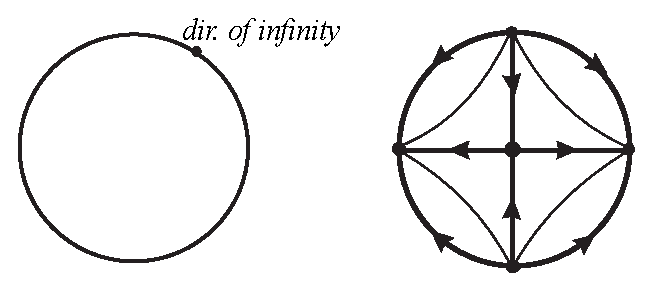
\includegraphics [scale=1]{jtr220}
		\caption{Poincaré plane}
		\label{fig:2.20}
\end{figure}

\begin{example}
	The linear vector field $\dot{x}=x,$ $\dot{y}=-y$ leads to a phase vector in the Poincaré plane as shown in Figure \ref{fig:2.20}.
\end{example}

\subsection{Orbital equivalence}

\begin{definition}
	Two vector fields $v (x)$ on $M$ and $w (y)$ on $N$ are \textbf{orbitally equivalent} if they have the same phase portraits from a topological point of view. It means, there is a homeomorphism $h:M\longmapsto N$ such that $h ($phase curve $v) = ($phase curve $w)$.
	The vector field $v (x)$ on $M$ is \textbf{orbitally structurally stable}, if every field $w(x)$ on $M$ sufficiently close to the field $v$ (in the appropriate topology) is orbitally equivalent to $v$.
\end{definition}

It is easy to see that, the above definition of orbital equivalence and orbital structural stability is weaker than the definition of equivalence and structural stability given in Definition \ref{def:1.24}.

Thus, the Hartman-Grobman's Theorem (Theorem \ref{theo:1.23}) and the following Proposition \ref{prop:1.25} show that two vector fields in the neighborhood of hyperbolic singular points with the same dimensions of a stable and unstable variety are orbitally equivalent. They are also orbitally structurally stable.

Below, without proof, we provide the necessary conditions for the orbital structural stability of a vector field on the plane.

\begin{theorem}\label{theo:2.43}
	If the field $v (x)$ in the area $U\subset \mathbb{R}^{2}$ is orbitally structurally stable, then:
	\begin{enumerate}[(i)]
		\item its singular points are hyperbolic,
		\item its closed phase curves are hyperbolic limit cycles,
		\item there are no separatrix connections.
	\end{enumerate}
	Moreover, if the area $U$ is compact (e.g. Poincaré plane), then the above conditions for orbital structural stability are also sufficient.
\end{theorem}

\subsection*{Tasks}
\begin{task}
	Calculate the solution of the system $\dot{x}=y,$ $%
	\dot{y}=-\sin x$ (mathematical pendulum) with the initial condition $%
	x(0)=0,$\ $y(0)=2$ corresponding to $H = 1$.
\end{task}

\begin{task}
	Similarly to the mathematical pendulum, find the first integral and sketch the phase curves for the \textit{Duffing system}
	$$
	\dot{x}=y,\text{ \ }\dot{y}=-x+x^{3}.
	$$
	Calculate the solution with the initial condition $x(0)=0,$ $y(0)=1/%
	\sqrt{2}$.
\end{task}

\begin{task}
	Calculate $\dot{r}$ and in $\dot{\varphi}$ Example \ref{example:2.4}.
\end{task}

\begin{task}
	Show that the value of the matrix $A$ in the transformation of Poincaré return $f (z) = Az +\ldots$ does not depend on the choice of cutting $S$ to the periodic orbit $\gamma .$
\end{task}

\begin{task}
	Prove formula \eqref{2.4}.
\end{task}

\begin{task}
	Calculate the coefficient $a_1$ in formula \eqref{2.6}.
\end{task}

\begin{task}
	Assuming that on the right side of the equation \eqref{2.7} there are only square terms (i.e. $D = E =\ldots = 0$) and that $c_3 = 0$, calculate $c_5$.
\end{task}

\begin{task}
	Show that for a linear vector field the number of limit cycles is 0.
\end{task}

\begin{task}
	Show that the $\omega$-limit set $\omega(x)$ for the stream $\left\{ g^{t}\right\} $ is closed and invariant, i.e., $g^{t}\left( \omega (x)\right) =\omega (x)$.
\end{task}

\begin{task}
	Show that in the proof of Theorem \ref{theo:2.19}, the consecutive points $x_j$ of the trajectory $\Gamma(x)$ of the point $x$ with the cutting $S$ form a monotonic sequence, as in Figure \ref{fig:2.7}.
\end{task}

\begin{task}
	Show that the vector field \eqref{2.11} has the property that the square of the radius $r^{2}=x^{2}+y^{2}$ grows along the solution for small $r$.
\end{task}

\begin{task}
	Calculate the index in $(0, 0)$ for the following fields:
	\begin{enumerate}[(a)]
		\item $\dot{x} = x^{3}-3xy^{2},\text{ \ }\dot{y}=y^{3}-3x^{2}y$
		\item $\dot{x} = y+x^{2},\text{ \ \ }\dot{y}=x^{3}$
	\end{enumerate}
\end{task}

\begin{task}
	Show that $i_{0}v=\textrm{sign}\det A$ for the field germ $\dot{x}=Ax+\ldots $ in $\left( \mathbb{R}^{n},0\right) $ such that $\det A\not=0.$ Note: the case of $n> 2$ is a task with an asterisk.
\end{task}

\begin{task}
	Show that the vector field $\dot{x}=1-xy,$ $%
	\dot{y}=x$ does not have limit cycles.
\end{task}

\begin{task}
	Show that the characteristic exponent of the periodic orbit defined in Definition \ref{def:2.27} is well defined.
\end{task}

\begin{task}
	Complete the analysis of the Jouanolou system in the case of the odd $s$.
\end{task}

\begin{task}
	Calculate \textrm{div}$\left( \frac{1}{f}v\right) $ in Van der Pol's analysis.
\end{task}

\begin{task}
	Sketch a phase portrait (in $\mathbb{R}^{2}$) for the system $\dot{x}=1+x^{2}-y^{2},$\ $\dot{y}=x+x^{2}-2xy.$
\end{task}

\begin{task}
	Sketch a phase portrait for the system $\dot{x}%
	=y^{2}-4x^{2},$ $\dot{y}=4y-8.$
\end{task}

\begin{task}
	Sketch a phase portrait for the equations $\dot{z}=z^{2}$ and $\dot{z}=\bar{z}^{2},$ where $z=x+iy\in \mathbb{C}\simeq
	\mathbb{R}^{2}.$
\end{task}

\begin{task}
	Consider the vector field $v (x, y)$ of form \eqref{1.2}, i.e., $\dot{x}=y+x^{2},$ $\dot{y}=-2x^{3}-4xy-y(x^{2}+y^{2})^{2};$ we want to show that the phase portrait of this circuit is as in Figure \ref{fig:1.2}.
	\begin{enumerate}[(a)]
		\item Let's start with the simpler vector field $v_{0}(x,y)$ given by the system\begin{equation}
		\label{2.17}
		\dot{x}=y,\ \ \ \dot{y}=-2x^{3}-4xy.
		\end{equation}
		Make a substitution with $z=x^{2}$ to sketch its phase portrait and show that in the neighborhood $x=y=0$ it is of the same quality as in Figure \ref{fig:1.2} (only has a larger elliptic sector). Also indicate that the parabola $y=-x^{2}$ is invariant for the field \eqref{2.17} and contains separators at the hyperbolic boundary.
		\item Using double blow show, the fields $v$ and $v_0$ have the same phase portrays in the neighborhood $x = y = 0$.
		\item Show that adding the component $-y\left(
		x^{2}+y^{2}\right) ^{2}\frac{\partial }{\partial y}$ of the field $v_{0}$ causes that in the area $U=\left\{ y\geq -x^{2}\right\} $ (i.e. the whole elliptic sector for $v_{0}$ with the edge) we divide the phase curves of the field $v_{0}$ by the angle, and so that the phase curves of the field $v$ move more toward the center of the coordinate system. In conclusion, all points in the area $U$ go to $(0, 0)$ under the influence of the phases $\left\{ g_{v}^{t}\right\}_{t>0}$.
		\item Show that the remaining points from the neighborhood of $(0, 0)$ either lie in the stable separatrix of the point $(0, 0)$ (i.e., for $v$) or enters the domain $U$ after the end of time under the influence of the stream $g_{v}^{t}.$
	\end{enumerate}
\end{task}